\documentclass[12pt,a4paper,oneside]{report}             % Single-side
%\documentclass[11pt,a4paper,twoside,openright]{report}  % Duplex


\usepackage{ifxetex}
\ifxetex
  \usepackage{fontspec}
\else
  \usepackage[T1]{fontenc}
  \usepackage[utf8]{inputenc}
  \usepackage{lmodern}
\fi

\usepackage[magyar]{babel} % Alapértelmezés szerint utoljára definiált nyelv lesz aktív, de később külön beállítjuk az aktív nyelvet.

\usepackage{combelow}
\usepackage{newunicodechar}

\newunicodechar{Ș}{\cb{S}}
\newunicodechar{ș}{\cb{s}}
\newunicodechar{Ț}{\cb{T}}
\newunicodechar{ț}{\cb{t}}

\usepackage{cmap}
\usepackage{amsfonts,amsmath,amssymb} % Mathematical symbols.
\usepackage[ruled,boxed,resetcount,linesnumbered]{algorithm2e} % For pseudocodes.
\def\algorithmcfname{algoritmus}
\makeatletter
\renewcommand{\fnum@algocf}{\AlCapSty{\AlCapFnt\thealgocf.\nobreakspace\algorithmcfname}}
\makeatother

\usepackage{booktabs} % For publication quality tables for LaTeX
\usepackage{graphicx}
\usepackage{sidecap}

%\usepackage{fancyhdr}
%\usepackage{lastpage}

\usepackage{anysize}
\usepackage{sectsty}
\usepackage{setspace}  % Ettol a tablazatok, abrak, labjegyzetek maradnak 1-es sorkozzel!

% For hyperlinks in the generated document. 
\usepackage{color}
\usepackage{listings} % For source code snippets.

%\usepackage[amsmath,thmmarks]{ntheorem} % Theorem-like environments.

\usepackage[hang]{caption}
\usepackage{scrextend}

\usepackage{indentfirst}
\usepackage{pdfpages}

\usepackage{xfrac}
\usepackage{eurosym}

\usepackage{fullpage} % a margokra is lehessen irni

\newcommand{\vigyazat}{\marginpar{\textcolor{red}{\emph{Vigy\'azat!}}}}

\usepackage{tikz}
\usepackage{verbatim}
\usetikzlibrary{arrows,shapes}
\usetikzlibrary{positioning}
\tikzset{main node/.style={circle,fill=blue!20,draw,minimum size=1cm,inner sep=0pt},
}

%--------------------------------------------------------------------------------------
% Language configuration -- choose one
%--------------------------------------------------------------------------------------
%--------------------------------------------------------------------------------------
% Elnevezések
%--------------------------------------------------------------------------------------
\newcommand{\dolgozatnyelve}{\selectlanguage{magyar}}



\newcommand{\bsc}{Diplomadolgozat}
\newcommand{\msc}{Disszert\'aci\'os dolgozat}

\newcommand{\pelda}{Példa}
\newcommand{\definicio}{Definíció}
\newcommand{\tetel}{Tétel}

\newcommand{\bevezeto}{Bevezető}
\newcommand{\koszonetnyilvanitas}{Köszönetnyilvánítás}
\newcommand{\abrakjegyzeke}{Ábrák jegyzéke}
\newcommand{\tablazatokjegyzeke}{Táblázatok jegyzéke}
\newcommand{\irodalomjegyzek}{Irodalomjegyzék}
\newcommand{\fuggelek}{Függelék}


\newcommand{\englishParagraph}{
	\setlength{\parindent}{0em} % angol nyelvű dokumentumokban jellemző
	\setlength{\parskip}{0.5em} % angol nyelvű dokumentumokban jellemző
	\nonfrenchspacing
}

\newcommand{\hungarianParagraph}{
	\setlength{\parindent}{2em} % angol nyelvű dokumentumokban jellemző
	\setlength{\parskip}{0em}   % angol nyelvű dokumentumokban jellemző
	\frenchspacing
}

\newcommand{\defaultParagraph}{
	\hungarianParagraph
}  % Beállítások magyar nyelvű dolgozathoz

%--------------------------------------------------------------------------------------
% Main variables
%--------------------------------------------------------------------------------------



% Szak alapkepzes vagy mesteri
\newcommand{\szakHU}{INFORMATIKA SZAK} % SZOFTVERFEJLESZTES
\newcommand{\szakRO}{SPECIALIZAREA INFORMATIC\v A} % SPECIALIZAREA DEZVOLTAREA APLICA\c TIILOR SOFTWARE
\newcommand{\szakEN}{COMPUTER SCIENCE SPECIALIZATION} %SOFTWARE DEVELOPMENT SPECIALIZATION


\newcommand{\dolgozattipusHU}{DIPLOMADOLGOZAT} % MESTERI DISSZERT\'ACI\'O
\newcommand{\dolgozattipusRO}{LUCRARE DE DIPLOM\v A} %TEZA DE MASTERAT
\newcommand{\dolgozattipusEN}{BACHELOR THESIS} % MASTER THESIS

\newcommand{\szerzo}{Tankó Tamás} % Szerző neve
\newcommand{\temavezetoA}{Dr. Kátai Zoltán}
 

% Fokozatok

%Egyetemi tan\'ar/ Profesor universitar/Full Professor
%Egyetemi docens/ Conferențiar universitar/Associate professor
%Egyetemi adjunktus/Lector universitar sau Șef de lucrări /Lecturer
%Egyetemi tan\'arseg\'ed/Asistent universitar/Assistant professor


\newcommand{\temavezetoAfokozat}{Egyetemi docens}% Első konzulens neve
\newcommand{\temavezetoAfokozatRo}{Conferențiar universitar}
\newcommand{\temavezetoAfokozatEn}{Associate professor}
\newcommand{\temavezetoB}{Oltean-Péter Boróka}
\newcommand{\temavezetoBfokozat}{Egyetemi tan\'arseg}
\newcommand{\temavezetoBfokozatRo}{Asistent universitar}
\newcommand{\temavezetoBfokozatEn}{Assistant professor}% Második konzulens neve; hagyd üresen, ha egy konzulensed van.
\newcommand{\cimHu}{Szociális jelenségek vizsgálata egy valós cég email kommunikációs hálózatán} % Cím
\newcommand{\cimRO}{Studierea fenomenelor sociale într-o rețea de comunicare prin email a unei companii reale}
\newcommand{\cimEN}{Examining social phenomena in a real company's email communication network}
\newcommand{\ev}{2023} %az aktualis ev

%--------------------------------------------------------------------------------------
% Page layout setup
%--------------------------------------------------------------------------------------
% we need to redefine the pagestyle plain
% another possibility is to use the body of this command without \fancypagestyle
% and use \pagestyle{fancy} but in that case the special pages
% (like the ToC, the References, and the Chapter pages)remain in plane style

\usepackage{smartdiagram}
\usepackage{tikz,pgf}
\usepackage{pgfplots}
\pgfplotsset{width=7cm,compat=1.8}
\usetikzlibrary{matrix,calc,shapes}

\tikzset{
	treenode/.style = {shape=rectangle, rounded corners, draw, anchor=center, text width=5em, align=center, top color=white, bottom color=blue!20,inner sep=1ex},
	decision/.style = {treenode, diamond, inner sep=0pt},
	root/.style = {treenode, font=\Large, bottom color=red!30},
	env/.style = {treenode, font=\ttfamily\normalsize},
	finish/.style = {root, bottom color=green!40},
	dummy/.style = {circle,draw}
}


\setcounter{secnumdepth}{0}
\sectionfont{\large\upshape\bfseries}
\setcounter{secnumdepth}{2}

\sloppy % Margón túllógó sorok tiltása.
\widowpenalty=10000 \clubpenalty=10000 %A fattyú- és árvasorok elkerülése
\def\hyph{-\penalty0\hskip0pt\relax} % Kötőjeles szavak elválasztásának engedélyezése


%--------------------------------------------------------------------------------------
% Setup hyperref package
%--------------------------------------------------------------------------------------
\usepackage{xcolor}
\definecolor{bluecite}{HTML}{0875b7}
\usepackage[unicode=true,
bookmarksopen={true},
pdffitwindow=true, 
colorlinks=true, 
linkcolor=bluecite, 
citecolor=bluecite, 
urlcolor=bluecite, 
hyperfootnotes=false, 
pdfstartview={FitH},
pdfpagemode= UseNone]{hyperref}


%--------------------------------------------------------------------------------------
% Set up listings
%--------------------------------------------------------------------------------------



\definecolor{codegreen}{rgb}{0,0.6,0}
\definecolor{codegray}{rgb}{0.5,0.5,0.5}
\definecolor{codepurple}{rgb}{0.58,0,0.82}
\definecolor{backcolour}{rgb}{0.95,0.95,0.92}




\definecolor{lightgray}{rgb}{0.95,0.95,0.95}
\definecolor{darkgreen}{RGB}{3,125,80}
\lstset{frame=tb,
	language=Matlab,
	aboveskip=3mm,
	belowskip=3mm,
	showstringspaces=false,
	columns=flexible,
	basicstyle={\small\ttfamily},
	numbers=none,
	numberstyle=\tiny\color{gray},
	keywordstyle=\color{blue},
	commentstyle=\color{codegreen},
	%stringstyle=\color{mauve},
	breaklines=true,
	breakatwhitespace=true,
	tabsize=3,
	backgroundcolor=\color{lightgray},
}
\def\lstlistingname{k\'odr\'eszlet}	


%--------------------------------------------------------------------------------------
% Set up theorem-like environments
%--------------------------------------------------------------------------------------
% Using ntheorem package -- see http://www.math.washington.edu/tex-archive/macros/latex/contrib/ntheorem/ntheorem.pdf
%\swapnumbers
%\theoremstyle{plain}
%\theoremseparator{.}
\newtheorem{example}{\pelda}[section]

%\theoremseparator{.}
%\theoremprework{\bigskip\hrule\medskip}
%\theorempostwork{\hrule\bigskip}
%\theorembodyfont{\upshape}
%\theoremsymbol{{\large \ensuremath{\centerdot}}}
\newtheorem{definition}{\definicio}[section]

%\theoremseparator{.}
%\theoremprework{\bigskip\hrule\medskip}
%\theorempostwork{\hrule\bigskip}
\newtheorem{theorem}{\tetel}[section]

\newtheorem{conclusion}{Következtetés}[section]


%--------------------------------------------------------------------------------------
% Some new commands and declarations
%--------------------------------------------------------------------------------------
\newcommand{\code}[1]{{\upshape\ttfamily\scriptsize\indent #1}}
\newcommand{\doi}[1]{DOI: \href{http://dx.doi.org/\detokenize{#1}}{\raggedright{\texttt{\detokenize{#1}}}}} % A hivatkozások közt így könnyebb DOI-t megadni.

\DeclareMathOperator*{\argmax}{arg\,max}
%\DeclareMathOperator*[1]{\floor}{arg\,max}
\DeclareMathOperator{\sign}{sgn}
\DeclareMathOperator{\rot}{rot}


%--------------------------------------------------------------------------------------
% Setup captions
%--------------------------------------------------------------------------------------

\captionsetup[figure]{
	width=.75\textwidth,
	aboveskip=10pt}
\renewcommand{\captionlabelfont}{\bf}
%\renewcommand{\captionfont}{\footnotesize\it}


%--------------------------------------------------------------------------------------
% Redefine reference style
%--------------------------------------------------------------------------------------
\newcommand{\figref}[1]{\ref{fig:#1}.}
\renewcommand{\eqref}[1]{(\ref{eq:#1})}
\newcommand{\listref}[1]{\ref{listing:#1}.}
\newcommand{\sectref}[1]{\ref{sect:#1}}
\newcommand{\tabref}[1]{\ref{tab:#1}.}





%--------------------------------------------------------------------------------------
% Table of contents and the main text
%--------------------------------------------------------------------------------------

\begin{document}

% CIMOLDALAK
%~~~~~~~~~~~~~~~~~~~~~~~~~~~~~~~~~~~~~~~~~~~~~~~~~~~~~~~~~~~~~~~~~~~~~~~~~~~~~~~~~~~~~~
	%--------------------------------------------------------------------------------------
%	A magyar cimoldal
%--------------------------------------------------------------------------------------
\begin{titlepage}
	\begin{center}
	
		\large{\bfseries SAPIENTIA ERDÉLYI MAGYAR TUDOMÁNYEGYETEM} \\
		\large{\bfseries MAROSVÁSÁRHELYI KAR,} \\
		\large{\bfseries \szakHU} \\[2.5cm]
			\begin{center}
			
\includegraphics[scale=2]{images/sapientia-hu}
		\end{center}
		\vspace{0.3cm}
		\Large{\Large  \cimHu}\\[0.8cm]
		\vspace{0.2cm}
		\textsc{\Large \bfseries \dolgozattipusHU}\\[2.5cm]
		
		{
			\large
		
			\renewcommand{\arraystretch}{0.65}
			\begin{tabular}{cc}
				  \makebox[6.5cm]{Témavezetők:} & \makebox[6.5cm]{Végzős hallgató:} \\ \noalign{\smallskip}
				 \makebox[6.5cm]{\temavezetoA,}  & \makebox[6.5cm]{\szerzo} \\ {\temavezetoAfokozat} \\
				 \makebox[6.5cm]{\temavezetoB,} & \\ \makebox[6.5cm]{\temavezetoBfokozat}
			\end{tabular}
		}
		
		\vfill
		{\large \bfseries \ev}
	\end{center}
\end{titlepage}
	%--------------------------------------------------------------------------------------
%	The title page RO
%--------------------------------------------------------------------------------------

\begin{titlepage}
	\begin{center}
	
		\large{\bfseries UNIVERSITATEA SAPIENTIA DIN CLUJ-NAPOCA} \\
		\large{\bfseries FACULTATEA DE ȘTIINȚE TEHNICE ȘI UMANISTE,} \\
		
		\large{\bfseries \szakRO} \\[2.5cm]
		
			\begin{center}
			
\includegraphics[scale=2]{images/sapientia-ro}
		\end{center}
		
		\vspace{0.3cm}
		
	
		
		\Large{\Large \cimRO}\\[0.8cm]
		\vspace{0.2cm}
		\textsc{\Large \bfseries \dolgozattipusRO}\\[2.5cm]
		
		{
			\large
		
			\renewcommand{\arraystretch}{0.65}
			\begin{tabular}{cc}
				 \makebox[6.5cm]{Coordonator științific:} & \makebox[6.5cm]{Absolvent:} \\ \noalign{\smallskip}
				 \makebox[6.5cm]{\temavezetoA,}  & \makebox[6.5cm]{\szerzo} \\ {\temavezetoAfokozatRo} \\
				 \makebox[6.5cm]{\temavezetoB,} & \\ \makebox[6.5cm]{\temavezetoBfokozatRo}
			\end{tabular}
		}
		
		\vfill
		{\large \bfseries \ev}
	\end{center}
\end{titlepage}
	%--------------------------------------------------------------------------------------
%	The title page EN
%--------------------------------------------------------------------------------------

\begin{titlepage}
	\begin{center}
	
		\large{\bfseries SAPIENTIA HUNGARIAN UNIVERSITY OF TRANSYLVANIA} \\
		\large{\bfseries FACULTY OF TECHNICAL AND HUMAN SCIENCES} \\
		\large{\bfseries \szakEN} \\[2.5cm]
		
			\begin{center}
			
\includegraphics[scale=2]{images/sapientia-en}
		\end{center}
		\vspace{0.3cm}
		\Large{\Large  \cimEN}\\[0.8cm]
		\vspace{0.2cm}
		\textsc{\Large \bfseries \dolgozattipusEN}\\[2cm]
		
		{
			\large
	
			\renewcommand{\arraystretch}{0.2}
			\begin{tabular}{cc}
				 \makebox[6.5cm]{Scientific advisor:} & \makebox[6.5cm]{Student:} \\ \noalign{\smallskip}
				 \makebox[6.5cm]{\temavezetoA,}  & \makebox[6.5cm]{\szerzo} \\ {\temavezetoAfokozatEn} \\
				 \makebox[6.5cm]{\temavezetoB,} & \\ \makebox[6.5cm]{\temavezetoBfokozatEn}
			\end{tabular}
		}
		
		\vfill
		{\large \bfseries \ev}
	\end{center}
\end{titlepage}
	
	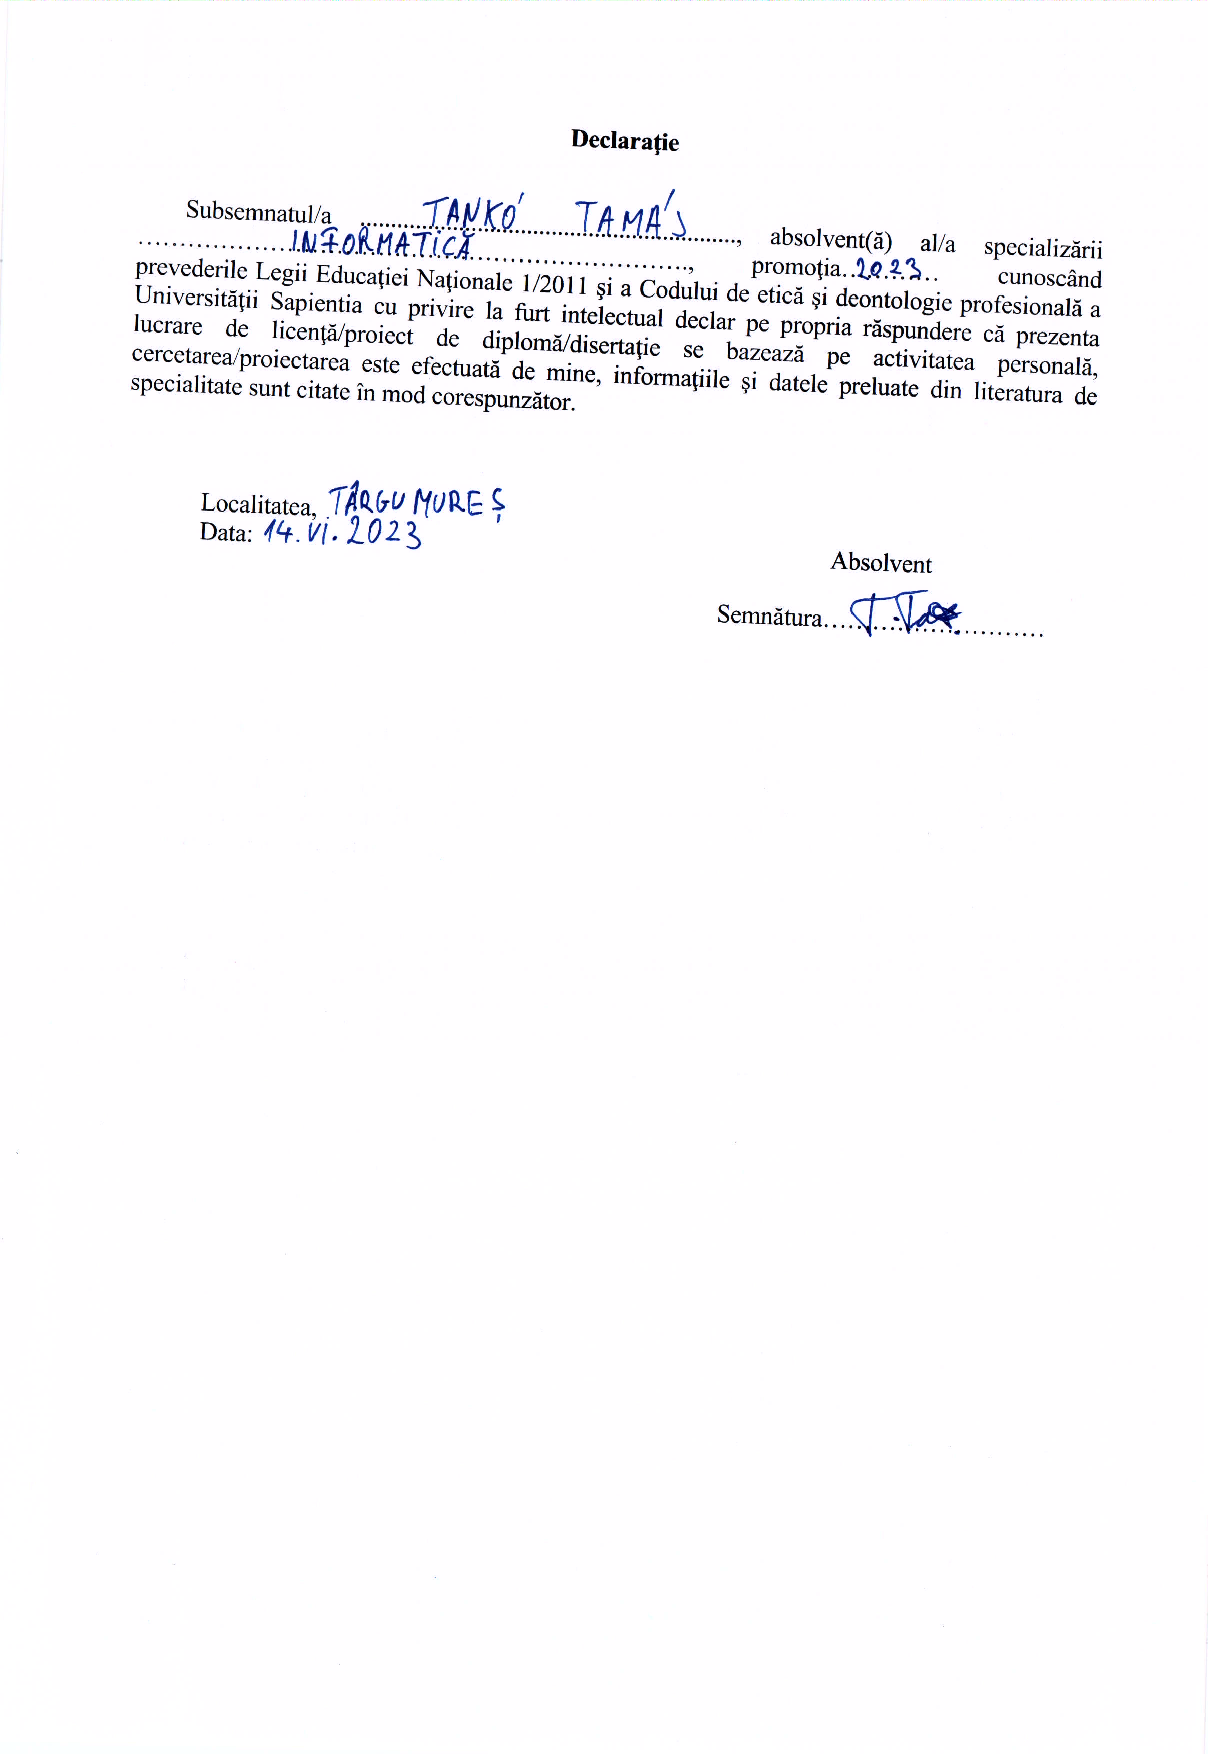
\includepdf[pages={1}]{content/declaratieTankoTamas.pdf}
	\pagenumbering{gobble}

\selectlanguage{magyar}
\hungarianParagraph

%----------------------------------------------------------------------------
% Abstract in Hungarian
%----------------------------------------------------------------------------

\chapter*{Kivonat}
Dolgozatom témája a szociális jelenségek vizsgálata egy valós cég e-mail kommunikációs hálózatán, amely során különböző gráfokra alkalmazott algoritmusok futásidejét hasonlítom össze. Ezen műveletekkel összekapcsolom a szociális jelenségeket az informatikai algoritmikával és gráfelmélettel. Előnyös esetként nem egy kitalált (fiktív) adatbázis elemeivel dolgoztam, hanem az ENRON valós e-mail kommunikációs adatbázisán végeztem. A kutatás során adatbányászatot végeztem el, hogy kizárólag a vállalaton belüli kapcsolatokat vizsgáljam meg, ezzel csökkentve a gráfban használt csúcsok számát.

Az interdiszciplináris kutatásom során különböző gráfelméleti algoritmusokat használtam, például a mélységi bejárás és a Girvan-Newman módszer.

A valós adatbázis lehetőséget nyújt a hálózat dinamikájának vizsgálatára, ezáltal a kapcsolatok kialakulása is követhető, amit vizualizálással is megjelenítek.


\vfill
\selectlanguage{romanian}

%----------------------------------------------------------------------------
% Abstract in Romanian
%----------------------------------------------------------------------------
\chapter*{Rezumat}

Románra fordítva: Tema lucrării mele este investigarea fenomenelor sociale într-o rețea de comunicare prin email a unei companii reale, în cadrul căreia compar duratele de execuție ale algoritmilor aplicați asupra diferitelor grafuri. Prin aceste operațiuni, conectez fenomenele sociale cu algoritmica informatică și teoria grafurilor. Într-un scenariu favorabil, nu am lucrat cu elemente fictive, ci am utilizat baza de date reală a comunicărilor prin email ale companiei ENRON. În cadrul cercetării, am efectuat și minerit de date pentru a examina exclusiv relațiile interne din cadrul companiei, reducând astfel numărul de noduri utilizate în graf.

În timpul cercetării mele interdisciplinare, am utilizat diferite algoritme de teoria grafurilor, precum parcurgerea în adâncime și metoda Girvan-Newman.

Baza de date reală oferă posibilitatea de a investiga dinamica rețelei, permițându-ne să urmărim formarea conexiunilor, care pot fi vizualizate.

\vfill
\selectlanguage{english}
%\englishParagraph

%----------------------------------------------------------------------------
% Abstract in English
%----------------------------------------------------------------------------
\chapter*{Abstract}


The topic of my paper is the examination of social phenomena in a real company's email communication network, where I compare the execution times of algorithms applied to different graphs. Through these operations, I connect social phenomena with computer algorithms and graph theory. In a favorable scenario, I did not work with fictional elements, but used the real email communication database of the ENRON company. In the research, I also conducted data mining to exclusively examine internal relationships within the company, thereby reducing the number of nodes used in the graph.

During my interdisciplinary research, I utilized various graph-theoretical algorithms such as depth-first search and the Girvan-Newman method.


The real database provides the opportunity to examine the dynamics of the network, allowing us to track the formation of connections, which can be visualized as well.


\vfill
\dolgozatnyelve
\defaultParagraph
 
% Tartalomjegyzek
%~~~~~~~~~~~~~~~~~~~~~~~~~~~~~~~~~~~~~~~~~~~~~~~~~~~~~~~~~~~~~~~~~~~~~~~~~~~~~~~~~~~~~~
	\pagenumbering{arabic}
	\setcounter{page}{9}
	\tableofcontents\vfill

% A diplomadolgozat lenyegi resze
%~~~~~~~~~~~~~~~~~~~~~~~~~~~~~~~~~~~~~~~~~~~~~~~~~~~~~~~~~~~~~~~~~~~~~~~~~~~~~~~~~~~~~~

% ajánlott külön file-okba írni az egyes fejezeteket, ugyanis úgy jobban át lehet látni.



	%----------------------------------------------------------------------------
\chapter{Bevezető}%\addcontentsline{toc}{chapter}{Bevezető}
%----------------------------------------------------------------------------

Az emberek életében létfontosságú a kapcsolatok fenntartása, ezáltal minden embernek létrejön egy szociálisan vizsgálható környezete, amelynek következménye egy hálózat létrejötte. Ezen hálózatok sokasága könnyen ábrázolható gráfként, amelyet különböző vizsgálatoknak lehet alávetni.
Az egyik legkiemelkedőbb mérési lehetőség a kapcsolatokban észlelhető hidak felismerése, valamint különböző algoritmusok alkalmazása a hálózaton (például a Girvan-Newman módszer).

A 21. században a számítógépekkel való kezelhetőség és a mérhetőség jelenti a legjellemzőbb képességet az emberi kapcsolatokból származó hálózatok szempontjából. Az egyik legjobb példa erre az internet, amelyet napjainkban több millió ember használ naponta. Ha elgondolkodunk ezen, láthatjuk, hogy az interneten keresztül létrejött hálózaton rengeteg adat és személy közötti kapcsolat tárolható. Az ilyen hálózatok elérhető adatainak kutatása ma népszerűvé vált, és több informatikai témakört egyesít.
Egy felhasználható valós adatbázis a kutatások szempontjából az Enron kommunikációs hálózata.\cite{Enron02}
Ezen adatbázist már többen kutatták, de én szerettem volna egy olyan kutatást végezni, amely hozzájárul az egyetemi tananyag bővítéséhez. Ezért átnéztem több kutatást \cite{Enron01}, és saját elképzelésem alapján alkalmaztam néhány algoritmust a kapott hálózaton.
Dolgozatom elkészítése során az algoritmusok összehasonlítása mellett adatbányászattal és kommunikációs hálózatok vizsgálatával is foglalkoztam. Minden hálózatnak megvannak sajátos tulajdonságai, amelyek alapján különböznek egymástól, és így kijelenthető, hogy bár lehetnek közös vonások, nem egyformák.

Az egyik szempont, amely alapján sorolhatóak a hálózatok, a kapcsolatok sűrűsége, azaz az általam választott esetben az Enron vállalatban dolgozók közötti üzeneteket tekintettem élnek a gráfokban. Mikor lesz egy kapcsolati hálózat, gráf sűrűsége a lehető legnagyobb? Egy adott gráfnak akkor lesz nagyobb sűrűsége, ha a csúcsok közötti élek száma közelíti a maximális értéket (Egy n csúcsból álló irányítatlan gráfnak maximálisan n*(n-1)/2 éle lehet).

A mérésekhez irányított gráfokként használtam fel az adatokat, ugyanakkor az adatbázis méretét a lehető legkisebbre próbáltam csökkenteni a cég által biztosított fiókok szempontjából. Az így kapott személyeket azonnal vizsgálatok alá lehetett helyezni, valamint az így nyert adatok egy részéből adatvizualizációt is létrehoztam a hálózat átláthatóságának érdekében.

%----------------------------------------------------------------------------
\section{Cím értelmezése és a kutatás célja} 
%----------------------------------------------------------------------------



A cím, "Szociális jelenségek vizsgálata egy valós cég e-mail kommunikációs hálózatán", felhívja figyelmünket arra, hogy ez a hálózat nem egy általunk tervezett gráfot hoz létre, hanem egy cég munkatársai között létrejövő kapcsolatokat ábrázol. Az e-mail alapján határozhatók meg a gráf élei, a küldő és címzett részek alapján.

De miért nevezzük szociális jelenségek vizsgálatának ezt a kutatást?
Ez nagyon egyszerű válasz. Mivel az e-mailen keresztül történő kapcsolat emberi interakciókat foglal magába. Az így kialakult kapcsolatokban számos szociális jelenség jelentkezhet, például:
\begin{itemize}
    \item kommunikációs minták,melyre egy jó illusztráció, ha egy személy előnybe részesiti egy bizonyos csoporttal a kapcsolattartást.
    \item informacióáramlás és annak hatása, tehát egy emberi véleményt is befolyásolhat különboző  üzenetben szereplő informació
    \item társas támogatás és kapcsolatépités, ezen jelenség  arra mutat rá, hogy az üzenetváltásokkal tudjuk támogatni egymást, vagy szoros kapcsolatokat is tudunk kialakítani
    \item utolsó példaként a hálózati struktúrát sorolnám fel, amelyet én is választottam ezen kapcsolati lánc ellemzésére.
\end{itemize}


Miért választottam a hálózati struktúrát a szociális jelenségek közül?

A hálózatokat átalakíthatjuk gráfokká, ezáltal a jelenségek kutathatóak és vizsgálhatóak gráfelméleti szinten. Így a szociális jelenségeket összekapcsolhatom az informatikával, amelynek tudományával az elmúlt években foglalkoztam.

A kutatás célja, hogy létrehozzak egy olyan programot, amely megtalálja a legfontosabb személyt ebben a hálózatban, valamint meghatározza a hidakat, amelyek nélkül a hálózat több részre szakadna. A program fejlesztésével segíteni szeretnék az informatikát tanuló diáktársaknak, hogy valós cégből származó adathálózattal dolgozhassanak, és ne kelljen kitalálniuk egy adott gráfot. Emellett néhány vizualizált eredménnyel is szolgálni szeretnék a Girvan-Newman módszer alkalmazásával.

	%\include{fejezet3}
	%----------------------------------------------------------------------------
\chapter{A hálózat vizsgálatának lépései}
%----------------------------------------------------------------------------
A hálózat vizsgálatát több részre osztottam, mivel különböző programozási nyelveket használtam az eredmények kimutatásához.

Az alábbi ábra szemlélteti a kutatási folyamat lépéseit:


\begin{figure}[h]
	\centering
	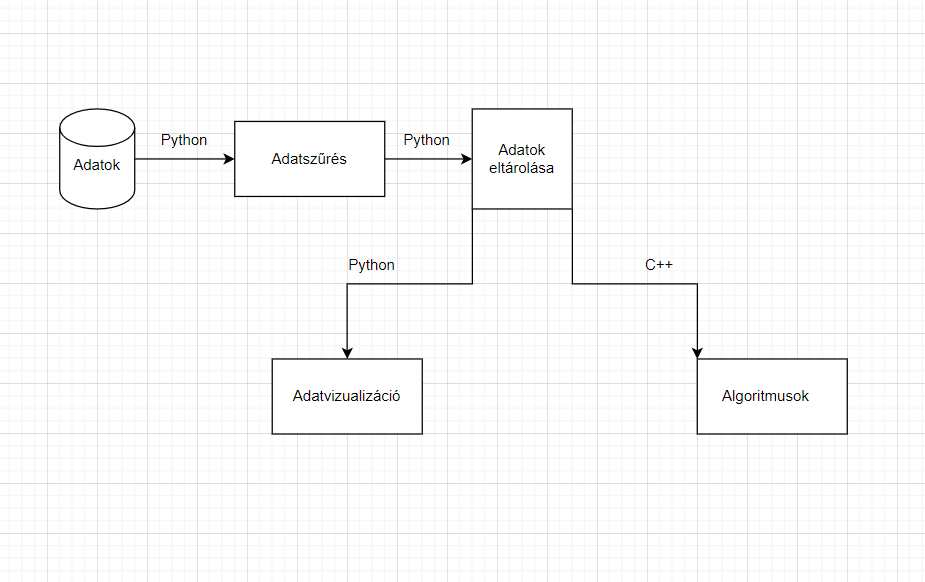
\includegraphics[scale=0.7]{images/lepesek}
	\caption{Folyamat ábra}
\end{figure}
\begin{itemize}
    \item Első lépésként az adatszűrés , adatbányászat , amely következtében feldolgozható adatokat átállítottam elő és ezen lépés után két részre választottam a műveleteket.
    \item  Egyik rész az adatok vizualizációja. Itt kirajzolásra kerül a hálózat kis rész gráfja és annak fejlődése .
    \item Második részben pedig a gráfelméletben megjelenő szociális jelenségek vizsgálata és ahhoz köthető algoritmusok megírása volt a fő célpont.
\end{itemize}
 
A programozási nyelvekek közül két különböző nyelvet, Python-t és C++-ot választottam, és használtam az adatokkal való műveletek és vizsgálatok során. A Python egy interpretált nyelv, ami azt jelenti, hogy fordítás nélkül futtatható. Ezzel szemben a C++ nyelvű forráskódot gépi kóddá kell fordítani a futtatható állomány létrehozása érdekében. A Python dinamikusan típusos nyelv, ami azt jelenti, hogy a változók típusát futásidőben határozza meg, nem kell előre meghatároznunk. Ez a tulajdonság nem alkalmazható a C++ nyelvre, de érdemes megemlíteni, hogy a C++ egy hatékony nyelv, amely lehetővé teszi a hardverközeli programozást és a memóriakezelést precízen irányítja.

Miért választottam a Python és a C++ nyelveket a kutatás során? Először is, minden műveletet el lehetett volna végezni más nyelveken is. Például az adatokat adatbázisban tárolhatnánk és az adatbáziskezelő nyelvét, például SQL-t használhatnánk a műveletek végrehajtásához. Egy másik lehetőség az adatok feldolgozására és vizualizációjára az adatbázisból való lekérdezések segítségével. Azonban én a Python és a C++ nyelveket választottam, mert a gráfelméleti algoritmusokat C++ nyelven tanultam, amihez a diákok már korábban is kapnak betekintést középiskolai tanulmányaik során. Ezért egy olyan nyelvet választottam, amelyet már ismernek, és könnyen át tudják gondolni az algoritmusok lényegét, ahelyett, hogy egy új nyelvet kellene elsajátítaniuk a téma mellett.

Ezzel a döntéssel a diákoknak lehetőségük van jobban megérteni és követni a programozási részleteket, és könnyebben alkalmazni a gráfelméleti algoritmusokat a kutatás során.

\section {Adatbányászat, adatszűrés}


Az adatbányászathoz a Python nyelvet használtam, amely segítségével sikerült megszerezni az összes Enron cég által biztosított e-mail címet. Konkrétan 5653 e-mail cím van, amelyek "@enron.com" végződéssel rendelkeznek. A kommunikációs hálózat létrehozásához az üzenetek jelentik az építőelemet, tehát ki kellett bányásznom és el kellett mentenem az üzeneteket annak érdekében, hogy létrehozhassak egy gráfot, amelyet vizsgálhatok. A szűrés ebben az esetben fontos volt, hogy csak az Enron-os e-mailek közötti üzeneteket használjam fel, ezzel csökkentve az adatok méretét. Még így is rengeteg adatot kaptam, pontosan 88975 üzenetet, amelyekről csak a minimális információt (küldő, címzett és dátum) mentettem el.

\begin{figure}[h]
	\centering
	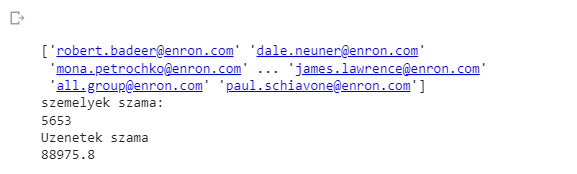
\includegraphics[scale=1]{images/adatokszama}
	\caption{Adatok számlálásának eredménye}
\end{figure}
\pagebreak%johet ide egy kodreszlet majd magyarazat  
 Az alábbi kódrészlettel kezdtem az adatokat kinyerni a megkapott adattömegből

\begin{figure}[h]
	\centering
	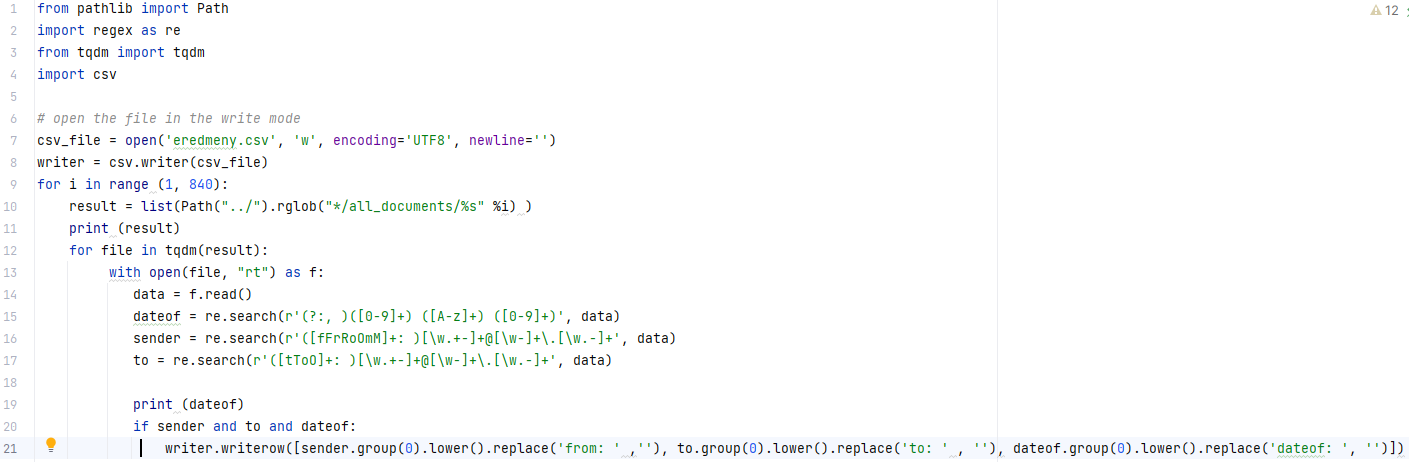
\includegraphics[scale=0.5]{images/adatbanyaszat}
	\caption{Adatbányászat}
\end{figure}

\begin{itemize}

        \item első lépésként létrehoztam egy csv fájlt, amelyben a megkapott adatokat tudom tárolni
	\item a következő lépés egy ciklus létrehozása, hogy minden személyt leellenőrizünk
	\item minden mappában több email szerepelt ezért először meghatároztam a fájlok listáját 
	\item ezen lista elemeit, tehát az összes fájlt meg kellett nyitnom és kikeresni a számomra szükséges adatokat(küldő,címzett és dátum)
	\item ezen adatok kiválasztásához regex kifejezéseket használtam amellyel nagyon egyszerűen lehetett rátaláni a helyes adatokra 
	\item minden olyan esetben ha volt dátum, küldő és címzett akkor az adathármast kiírattam a program elején létrehozott fájlba
        \item  ugyanakkor az itt kapott eredményt még át kellett futtatnom egy szűrési algoritmuson amelyet már az adatok biztonságos tárolása miatt Drive-ra töltöttem fel és onnan használtam fel .
         \item a szűréshez is Python nyelvet használtam amelyet már a gyors mentési lehetőséggel élve Colab-ban írtam meg.
         \item  a legfontosabb szempont az volt a helyes adatok kiválasztásában, hogy felhasználók e-mail címei "@enron.com"-végződéssel rendelkezzenek ugyanakkor az üzenetekben mindkét személyre jellemző legyen ezen tulajdonság.
\end{itemize}




\section {Adatvizualizáció}

A következő részben röviden bemutatom a hálózat megjelenítését és annak fejlődését.

Az ábrákon és adatokon, amelyeket eredményként bemutatok, az első 50 e-mail címet vettem figyelembe, valamint a közöttük lévő szigorú kapcsolatot és üzenetváltást. A vizualizáció előnye, hogy nem csak elképzelhetjük a kapcsolatok fejlődését, hanem ténylegesen láthatjuk azokat, és könnyebben észlelhetjük a változásokat.

A részhálózat megjelenítése előtt két műveletet hajtottam végre, amelyek segítették az algoritmusom gyorsabbá tételét.
\begin{itemize}
    \item Első művelet ,szűrés, amely fontos az optimálisabb futási időhöz , az adatok csökkentése, amelyet a következő ábrán látható program végezett el.
    \begin{figure}[!h]
        \centering
        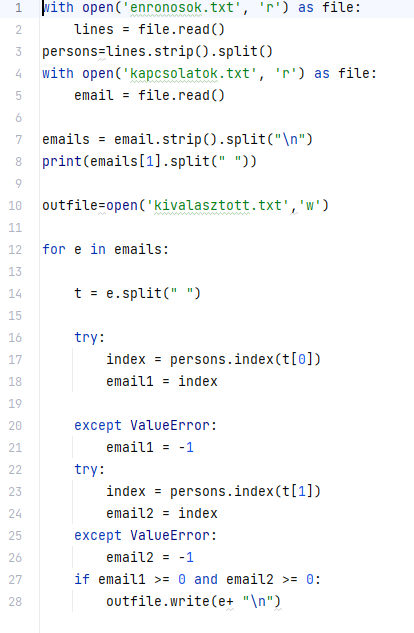
\includegraphics{images/kivalasztas}
        \caption{Szűrési művelet }    
    \end{figure}
    \begin{itemize}
        \item A fenti ábrán a program  megnyitja a 2 fájlt amelyben az adatok tárolva vannak, elsőben a személyeket tároltam, amiből tárolom egy tömbe az e-mail címeket, míg a második fájlból az üzenetek adatait fogom eltárolni .
        \item Harmadik fájlnévnél már láthatő hogy ezt fájlt nem olvasásra használom, mert ebbe fognak bekerülni a szűrésen áthaladó adatok egy része
        \item Számomra azon adatok kell hogy megmaradjanak, amelyek az első 50 személy közötti üzeneteket képezik 
        \item Ehhez a szürésnek köszönhetően elmondhatjuk hogy az 5653 felhasználóból kiválasztott első 50-hez nem 88976 üzenetet kell átnézek a következő adatvizualizációnál hanem csak 3969-et .
    \end{itemize}
    \item Második művelet ,rendezés, amely a kronológiai sorrendbe állítja az üzeneteket, kapcsolatokat, ehhez szükséges rendezést a képen látható kódrészlet által oldottam meg:
    \begin{figure}[!h]
        \centering
        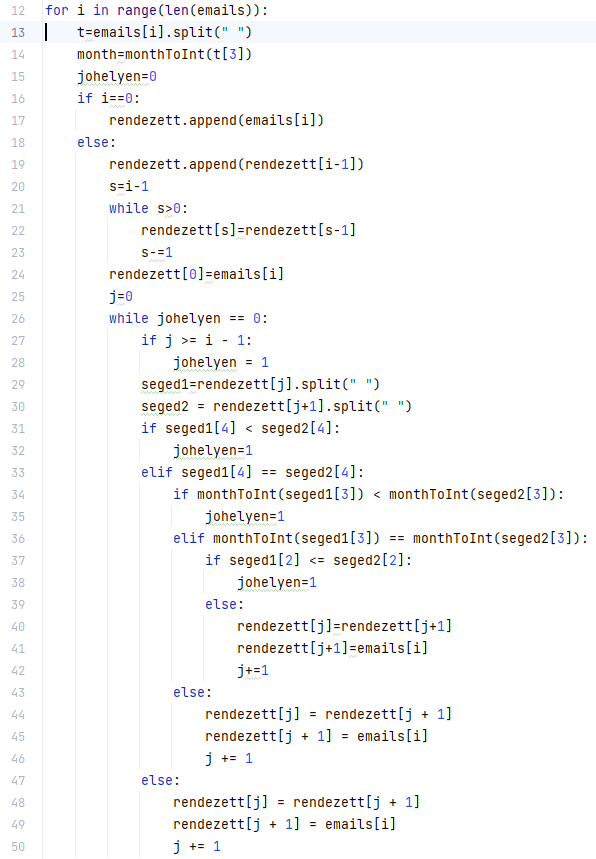
\includegraphics[scale=0.8]{images/rendezes}
        \caption{Rendezés kronológiailag}
        
    \end{figure}
    \item Az említett rendezési módszer, amit leírtál, hasznos a listaelemek sorba rendezésére. A módszeredben az elemeket egymással összehasonlítva és cserélve helyezed őket a megfelelő pozícióba. Emellett említetted, hogy egy saját függvényt használsz a hónapok helyes sorrendjének meghatározására.

Miután rendezted a listát, elmentetted az eredményt egy új fájlba, amit később felhasználhatsz az adatvizualizációhoz.

Ez a rendezési és mentési folyamat segít abban, hogy a hálózatot könnyebben áttekinthető és vizualizálható formában tudd megjeleníteni.
  
\end{itemize}
A szükséges adatcsökkentés és rendezés után következett a hálózat megjelenítése, amelyet az eddigi műveletekhez hasonló módon Pythonban készítettem el. Ez a kis rendszer egy felületet hoz létre, amely 1000 üzenet után frissíti a kapcsolati ábrát, így jól láthatók a különbségek akár 1000, akár 2000 üzenetküldés között. A rendezett e-mail lista segítségével ezek a változások idővel arányosan jelennek meg. Az alábbiakban látható a hálózat 1000 üzenet után, valamint a második képen az összes üzenet elküldése után.
\begin{figure}[h]
        \centering
        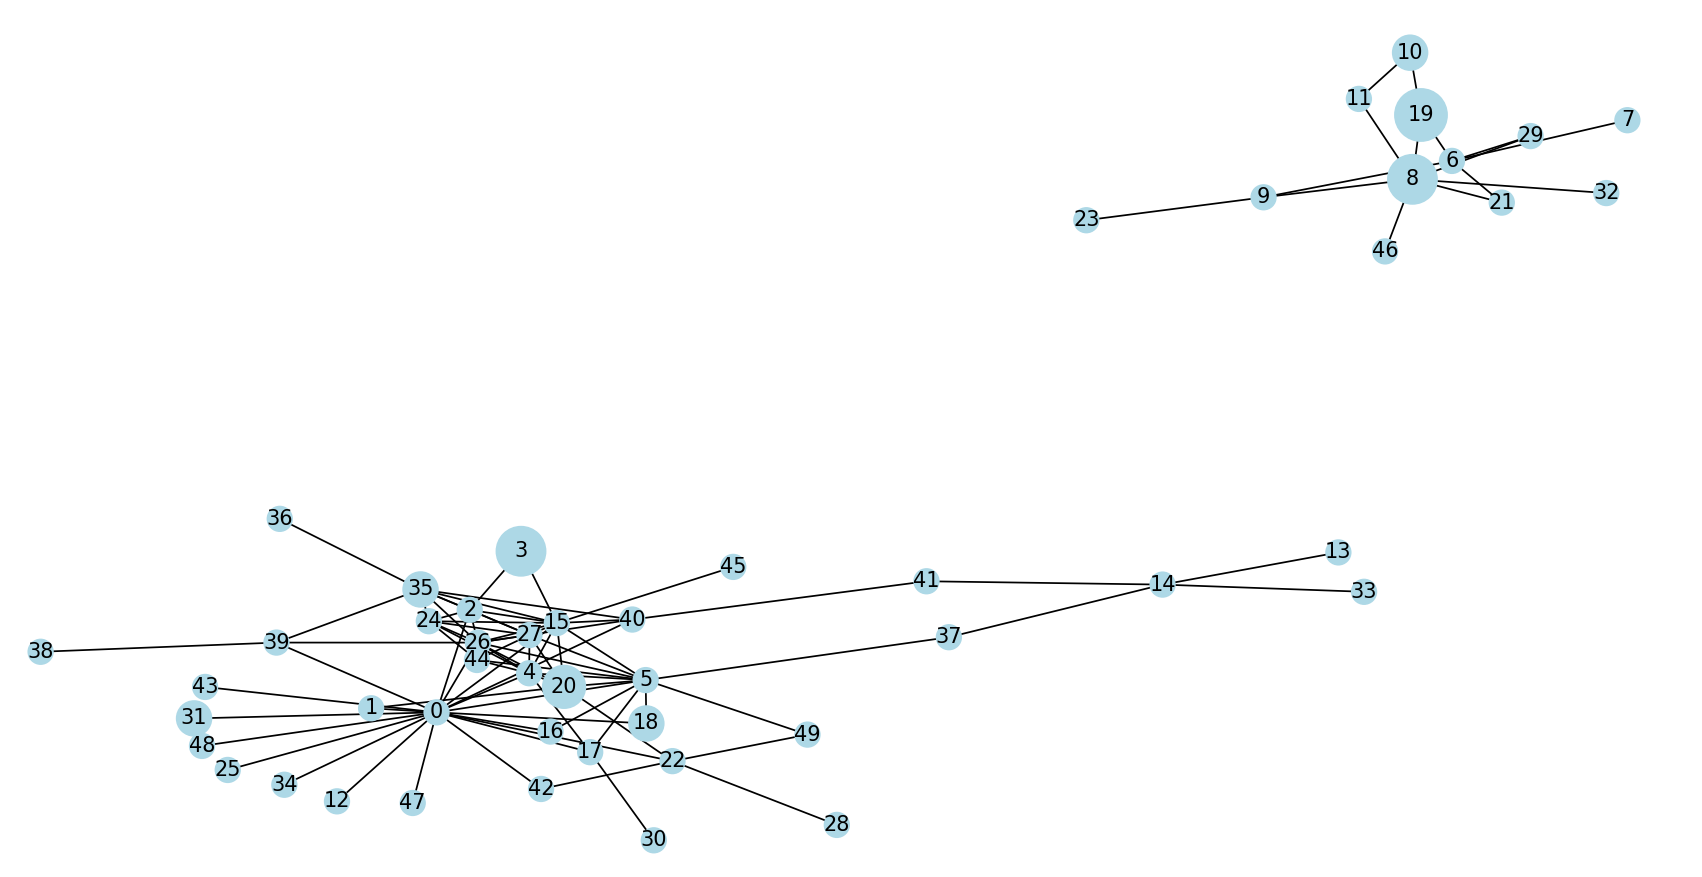
\includegraphics[scale=0.4]{images/elsorajz}
        \caption{1000 üzenet utáni hálózat}
        
    \end{figure}
    \begin{figure}[h]
        \centering
        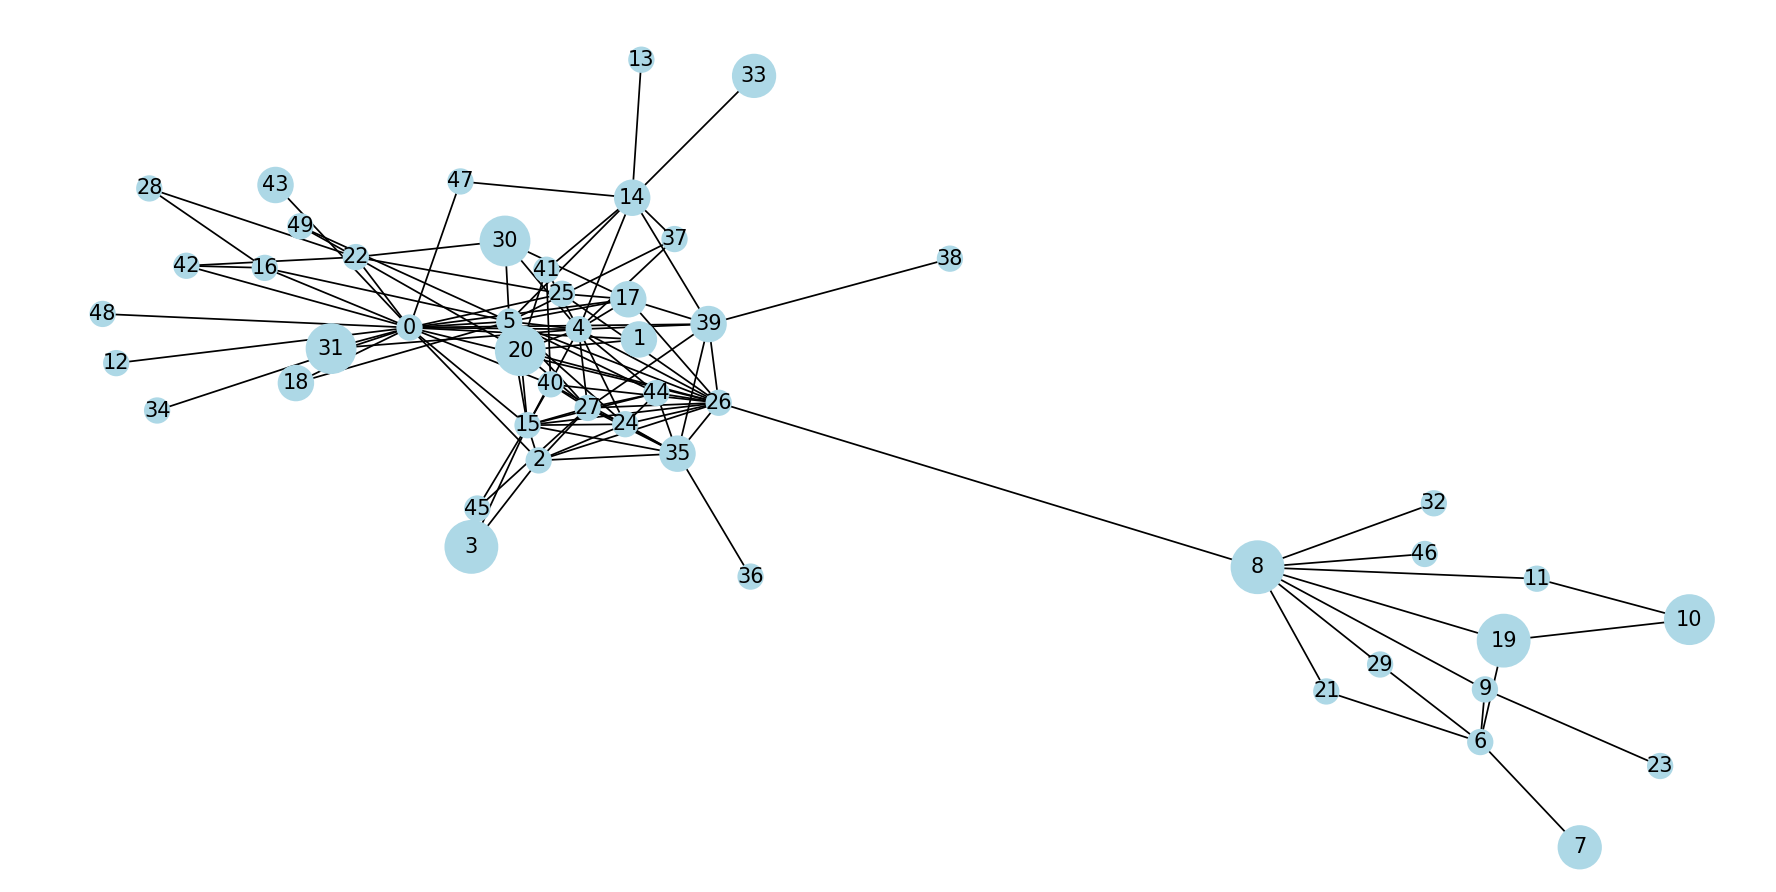
\includegraphics[scale=0.35]{images/utolsorajz}
        \caption{Összes üzenet utáni hálózat }
        
    \end{figure}

Az ábrákon észrevehető , hogy különböző méretűek a csúcspontok , amelyek az elküldött üzenetekkel arányosan növekednek .Ezen méretbeli eltérést az alábbi kód segítségével állítottam be:
\begin{figure}[h]
    \centering
    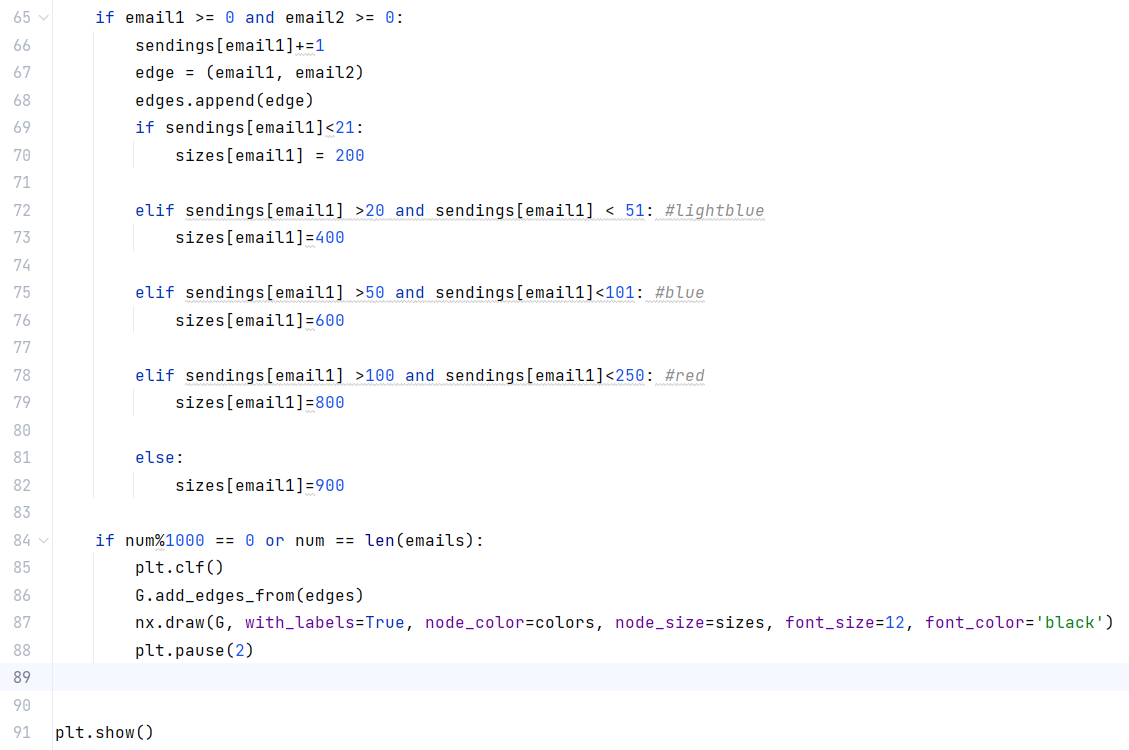
\includegraphics[scale=0.5]{images/vizualizacioskod}
    \caption{Csucspontok méretének beállítása és kijarzolása}
    \label{fig:enter-label}
\end{figure}

A kódrészletben feltüntetett 65. sorban látható egy ellenőrzés/feltétel, amelyben megnézem, hogy mindkét e-mail cím létezik-e. Ezen lépés után mindig a küldő résznél növelem az elküldött üzenetek számát, amelyet egy 50 elemű tömbben tárolok, és ezáltal tudom meghatározni, hogy az adott személy mikor kerül más területre, mikor kell növelnem az ő vizuális méretét. Ugyanakkor látható egy másik dinamikus tömb (edges névvel), amelyben számpárokat, pontosabban a gráf éleit tárolom.

Ha végeztünk az összes üzenettel, akkor a feltöltött tömbök segítségével létrehozzuk a gráfot. A tömb feltöltése több részben fog történni, mert így a kapcsolatok létrehozása során lehet kirajzoltatni a gráfot. Az általam választott lépés 1000 egységnyi nagyságú, és 2 mp-ig tart, hogy kirajzolja a gráfot, majd a következő lépés, változat következik, addig amíg eléri az utolsó üzenet feldolgozását.

Utolsó lépésként az adatvizualizációt bővítettem egy irányított gráf kirajzolásával. Az eddig használt 50 fős hálózat kapcsolatai irányokkal ellátva, valamint ráközelítve a program által generált ábra sűrített részébe.

\begin{figure}[h]
    \centering
    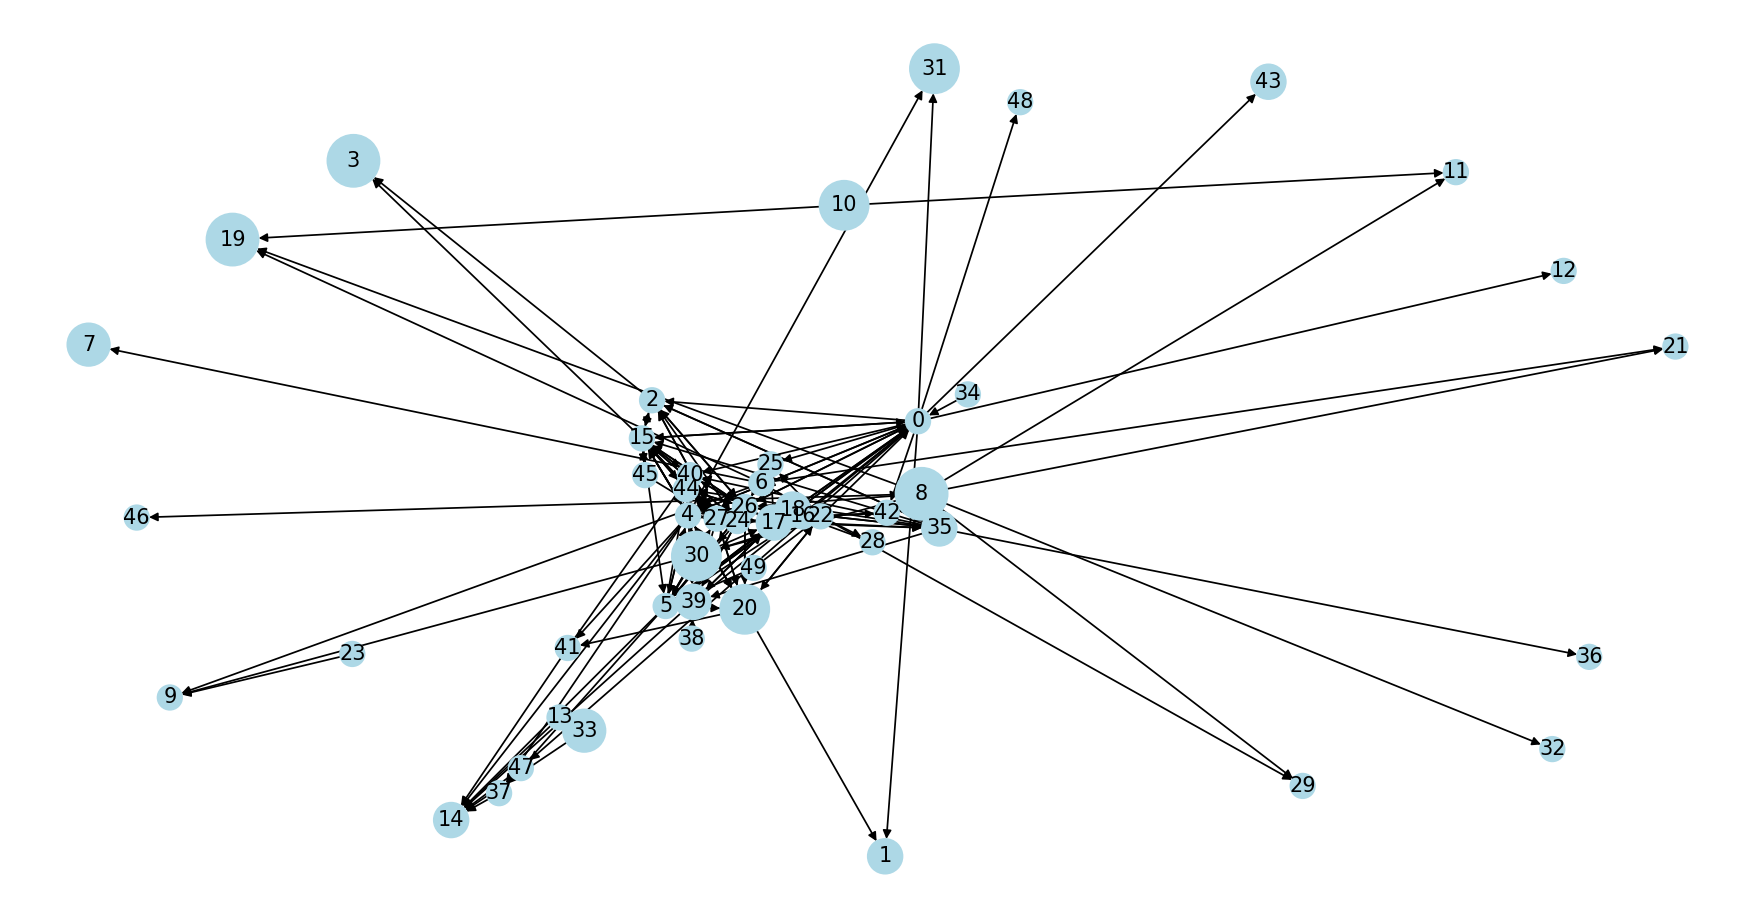
\includegraphics[scale=0.35]{images/iranyitott2}
    \caption{Csucspontok  kijarzolása irányított gráfként}
    \label{fig:enter-label}
\end{figure}
\begin{figure}[h]
    \centering
    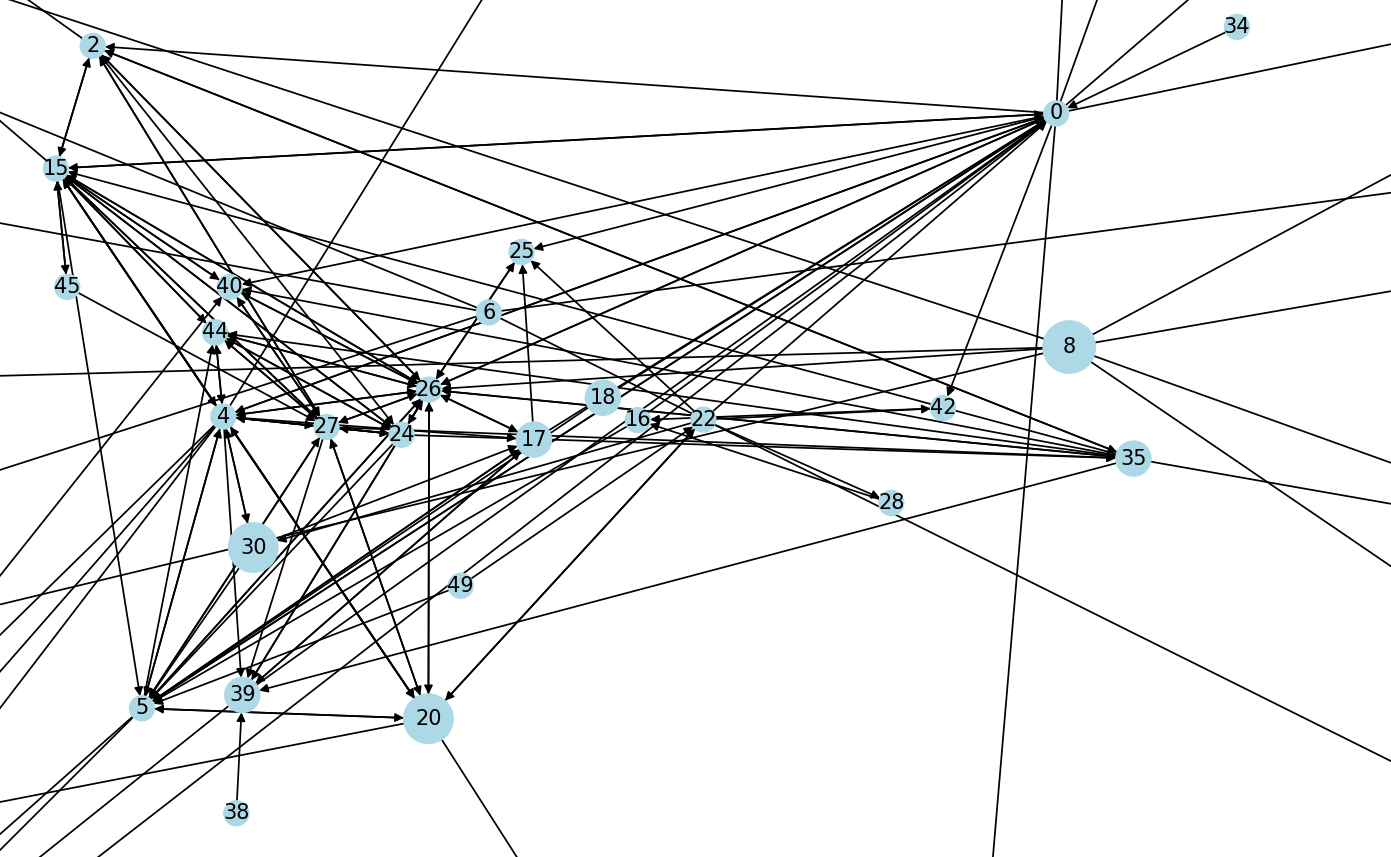
\includegraphics[scale=0.4]{images/iranyitott3}
    \caption{Kis nagyítás a gráf középpontjára}
    \label{fig:enter-label}
\end{figure}
\newpage
\section {Összességében}

A fenti esetekhez azért használtam a Python nyelvet, mert úgy éreztem, hogy ez az a nyelv, amely teljesen új volt számomra az egyetem kezdetén, valamint ezzel a nyelvvel könnyedén lehet adatokat szűrni, akár összehasonlítani egymással. Ugyanakkor nagyon sok könyvtárral rendelkezik a grafikonok vizualizációjához. Ezen könyvtárak közül választottam a Matplotlib-et, amely többek között támogatja a különböző diagramtípusokat, illetve lehetővé teszi a részletes testreszabást. Emellett nagyon elterjedt könyvtár, így rengeteg dokumentáció és példa áll rendelkezésre a különböző hibák kiküszöböléséhez.


	%----------------------------------------------------------------------------
\chapter{A hálózaton kipróbált algoritmusok}
%----------------------------------------------------------------------------
Ebben a fejezetben bemutatom az általam megírt algoritmusokat, amelyeket ezen hálózaton teszteltem, és egyben összehasonlítom egy méretben kisebb, fiktív gráfon is alkalmazva. Az algoritmusok programozási nyelve a C++, amely eltér az eddig használt nyelvtől. Ugyanakkor ezt a nyelvet választottam, mert ezeket a programokat később más diáktársak is felhasználhatják a gráfelméleti algoritmika elsajátításakor. Így viszonyítani tudom a sok fontos információt és tanácsot az egyetemnek, ha ez csak egy kis töredéke annak, amit én tanulhattam az elmúlt évek során.

Következzenek az általam megvalósított algoritmusok, amelyeket  a hálózat szociáis jellegű vizsgálatára készítettem :
\section{A pletyka terjedése}
\begin{figure}[!h]
	\centering
	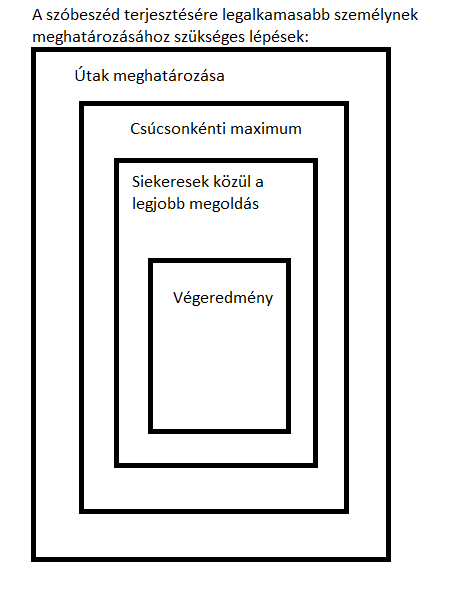
\includegraphics[scale=0.45]{images/elsoprogram}
	\caption{Szoftver lépései}
\end{figure}
Az első algoritmus a két pont közötti út meghatározására használt algoritmus továbbképzése, amelynek köszönhetően a szociológiai elemként tartott pletyka (szóbeszéd) milyen gyorsan tud terjedni, akár e-mailek által, egy nagyobb hálózaton keresztül.
Ezen program felépítése több lépésből áll, amelynek első lépése egy mélységi bejárás egy irányított gráfon, majd a második lépésben minden csúcsra meghatározzuk az utat, vagyis hogy az üzenet egyik személytől a másik személyig hány emberen keresztül jut el.

Ugyanakkor az utolsó lépésben meghatározom, hogy a hálózatban ki lenne a legjobb központ, ki által terjed a legjobban a pletyka, valamint melyik személy nem tudja eljuttatni mindenhová a szóbeszédet.

Látványos áttekintésként az alábbi gráfot hoznám fel, amely segítségével könnyebb megérteni a fent említett információkat.


\begin{figure}[!h]
	\centering
	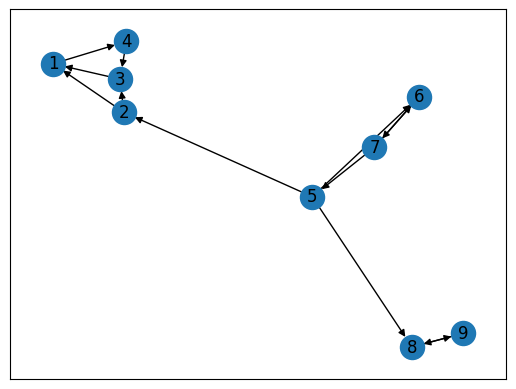
\includegraphics[scale=0.6]{images/kisgraf}
	\caption{Gráf a szóbeszédhez}
\end{figure}

Az ábrán látható egy 9 csúcspontból álló irányított gráf, amelyet azért készítettem, hogy érthetőbb legyen az algoritmus magyarázata.

Az első lépés a mélységi bejárás által meghatározni az utakat. A képen is látható, hogy az 1 pontból csak a 4 és 3 pontig jutunk el, tehát itt az üzenet csak 2 személyhez jut el. Hasonlóképpen nem jutunk messze a 2., 3. és 4. pontokkal sem. Az 5. pont már minden más csúcshoz el tudja küldeni az üzenetet. A leghosszabb út, amit megtesz az üzenet, a 4-es elemhez való információ közlést alkotja. Ehhez át kell mennie 2 ponton (2. és 1. csúcsokon), ami pontosan 3 él hosszú. Ezt a leghosszabb utat eltároljuk, valamint azt is, hogy összesen hány él mentén kellett bejárnia az utakat. Az utóbbi adat azért szükséges, ha van még egy hasonló elem, akkor ez dönti el, ki van a középpontban. De térjünk át egy másik olyan pontra, amely be tudja járni az egész gráfot, ez a pont a 7-es. A kiválasztott pont annyiban tér el az 5-östől, hogy a leghosszabb útja 4 él hosszú. Ezért a döntés az 5-ösre esik, így ő lesz a hálózat központja. Tehát az ő által küldött üzenetek érnek el mindenhová, és mindezt a legoptimálisabb idő alatt tudja elérni.

A kis példa után áttérnék az általam felhasznált 50 fős adattömegre, amelynek vizualizációját már bemutattam. Ugyanakkor bemutatom a programot, amelyet használtam az előző gráfnál is. Mint tudjuk, a gráfok nagysága és éleinek száma nagyban eltér, ezért összehasonlítottam a futási időket. A hamarosan megjelenített program a kis gráfra, amely 9 csúcsot és 12 élet tartalmaz, 0,0094 másodperc alatt végezte el a középpont megkeresését és annak pontos meghatározását, míg az 50 ezres és még szűrés nélküli, 80 000 fölötti üzeneteket tároló fájl használata során 0,0467 másodpercet volt képes elérni.

\newpage
Következzen is a C++ szoftver bemutatása és annak magyarázata:


\begin{figure}[!h]
	\centering
	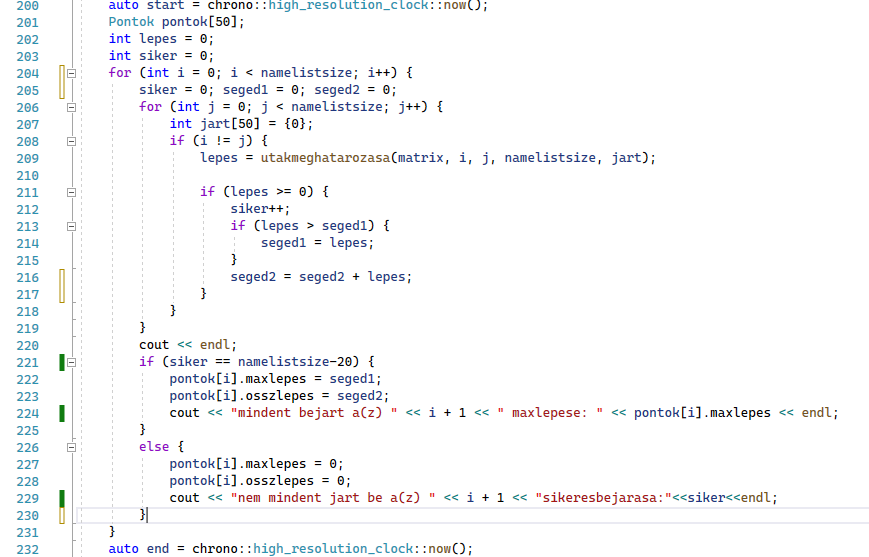
\includegraphics[scale=0.7]{images/utaskod}
	\caption{két pont közötti út távolság meghatározása}
\end{figure}

Az első képen látható egy függvény, amely, ahogy említésre került, az első lépésre íródott. Tehát meghatározza két pont között, hogy van-e út, és ha van, akkor az hány él hosszúsággal rendelkezik. Ennek a függvénynek összesen 5 paramétere van. Sorrendben egy két dimenziós tömb, tehát egy mátrix, majd az 'st' változó, amely egy valós számot tartalmaz, és a kezdő pontot határozza meg, vagyis hogy honnan kell indulni az út meghatározásához. A harmadik paraméter a végső pont indexét határozza meg, majd ezek után következik a méret, amely segíti a mátrix bejárását, és végül egy tömb, amelyben rögzítem, hogy az adott ponton már jártam-e. Ezzel a tömbbel ki tudom küszöbölni a gráfban keletkező körök létrejöttekor felmerülő végtelen ciklust.
A 't' és 'mint' változók a jelenlegi út hosszát tárolják, majd ezek közül a minimumot választják.

Kezdésként ellenőrzöm, hogy ha van kapcsolat az indulási pont és az úticél között, akkor megkapom, hogy az út hossza 1, és visszatérek vele. Ha nincs kapcsolat, akkor beállítom, hogy jártam a kezdő pontban, majd áttérek azokra az esetekre, amikor minden olyan útvonalat ellenőrzök, amely a kezdőpontból indul és valamerre halad. Ha nincs ilyen útvonal, akkor visszatérek -1 értékkel, amivel jelezem, hogy nincs út a két pont között. Ha van olyan eset, hogy a program tovább tud lépni a kezdőpontból, vagyis van kimenő éle a pontnak, akkor ebben az esetben hívom meg újra a függvényt, amikor már eljutottam a pozícióhoz. Ezzel a meghívással hozom létre a rekurziót.

A minimális út kiválasztása az alábbi módon történik: Ha már van értéke a 'mint' változónak, és nagyobb az eddig meghatározott útnál ('t'-nél), akkor megváltoztatom annak értékét. Ugyanakkor, ha a 'mint' változó továbbra is -1, és kapok egy helyes útvonalat, vagyis változott a 't' értéke, akkor visszaadom újra a 't' értékét. Abban az esetben, ha a 't' soha nem változik, akkor a 'mint' értéke változatlan marad, és a program -1 értéket térít vissza. De ha a 'mint' értéke változott, akkor az adott értékhez hozzáadok 1-et, és ezt a függvény visszatéríti, mivel ebben az esetben a következő ponttól volt számolva a távolság.

\newpage
\begin{figure}[h]
	\centering
	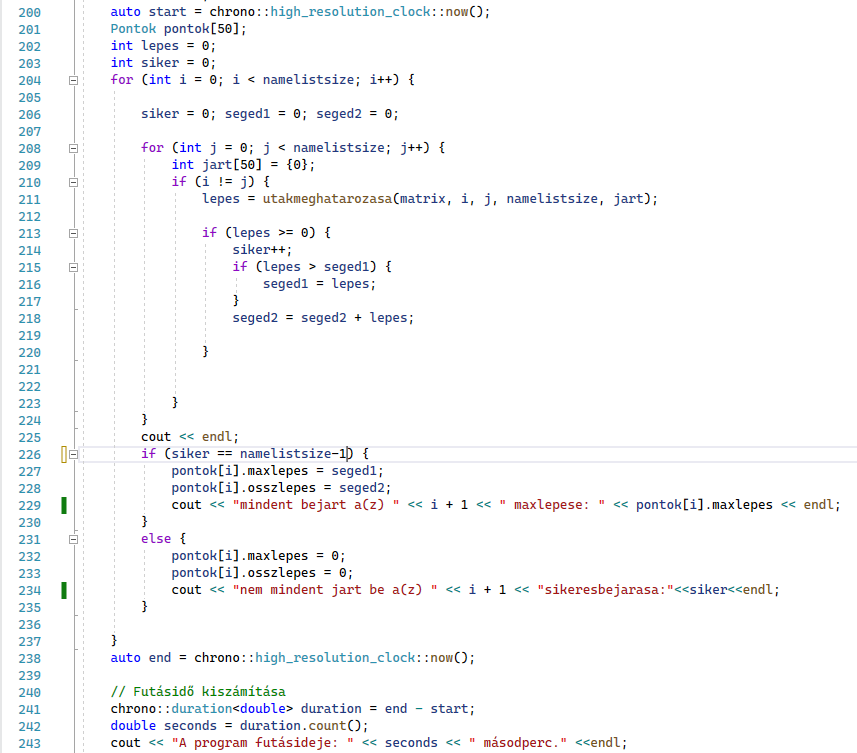
\includegraphics[scale=0.6]{images/kozeppont}
	\caption{Utak meghatározása és középső pont kiderítése}
\end{figure}

A fenti képen látható az algoritmus főbb része, amely során beolvasott adatokat feldolgozza a program, meghatározza minden csúcs által bejárt utak összegét, valamint ezek közül a legnagyobb út hosszát. Kivételt képeznek azok a csúcsok, amelyek nem tudnak üzenetet küldeni mindenkinek. A program minden érték esetén kiírja, hogy az adott személy elért-e mindenkit, és ha igen, akkor mekkora a maximális út, amit egy személy elérése során megtett.

A fenti képen látható, hogy az algoritmus futási ideje mérve van (200., 232. sor), és az eredményben is megjelenik ennek kiíratása.

\begin{figure}[h]
	\centering
	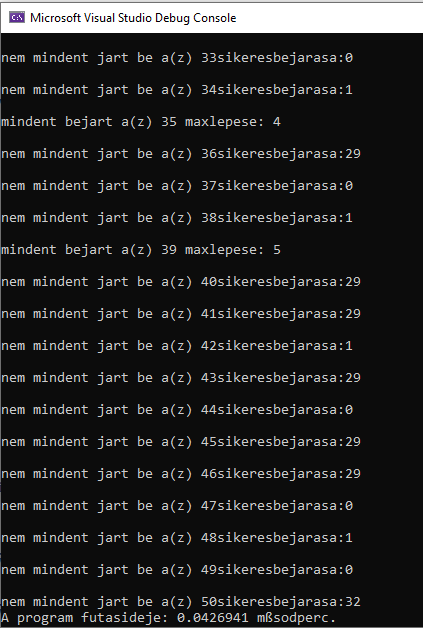
\includegraphics[scale=0.4]{images/utaseredmeny}
	\caption{Eredmény kiíratása}
\end{figure}

\section{A csomósodási együttható kiszámítása}

Mi az a csomósodási együttható? A csomósodási együttható egy érték, amely a gráfokban a csúcsokhoz kapcsolódik, és az adott pont szomszédok közötti kapcsolatot vizsgálja. Ez az érték egy aránynak tekinthető, amely maximum 1 lehet. Az arány két összetevőből áll: a szomszédok között lehetséges kapcsolatok száma és a létrejött kapcsolatok száma. A csomósodási együttható segítségével meg lehet határozni, hogy mennyi valószínűsége van annak, hogy egy pont barátai egymással is kapcsolatban állnak. Minél kevesebb szomszéddal rendelkezik egy csúcs, annál nagyobb az esélye annak, hogy közelíti az 1-hez tartó értéket.

Mi a csomósodási együttható célja? A csomósodási együttható mérése segít megérteni, hogyan változik a hálózat dinamikája az új élek hozzáadásával. Ha új élek kerülnek a gráfba, ez az érték növekedhet, és megfelelő mennyiségű él hozzáadásával általában eléri az 1-es értéket. Ha minden pont csomósodási együtthatója 1, akkor bármely pont kiválasztása esetén a szomszédok egy teljes gráfot alkotnak.

Összefoglalva, a csomósodási együttható az hálózat dinamikájának figyelésére szolgáló érték, amely rámutat a pontok közötti kapcsolatok kialakulására.

A használt hálózatot szép és látványos eredmények érdekében átalakítottam az irányított gráfból egy irányítatlan hálózattá. Ennek az átalakításnak az alapja az volt, hogy ha az x pont küld egy e-mailt az y pontnak, akkor az y pont ismeri az x pontot. Az alábbi ábrán bemutatom a szoftver lényeges részeit:
\begin{itemize}
    \item Kezdeném az elsődleges függvénnyel, amelyet a második lépésben felhasználok. Ez a függvény segít meghatározni az adott pont szomszédai között kialakult kapcsolatok, azaz élek számát. A függvény egy számot ad vissza, és a paraméterei között szerepel egy mátrix, amely tárolja a pontok közötti éleket. Emellett megkap egy tömböt is, amelyben szerepel a szomszédok listája, valamint a szomszédsági lista hossza is felhasználható harmadik paraméterként.

A függvény a mátrix bejárása során meghatározza, hány él található a szomszédok között, és ezt az értéket az 'eredmény' változóban tárolja. Ezután az eredményt visszatéríti.
    \begin{figure}[h]
    \centering
    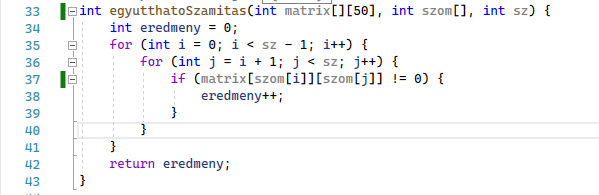
\includegraphics[scale=1 ]{images/egyutthatoszamitas}
    \caption{Együttható kiszámításához használt függvény}
    \end{figure}
    
    \item A második kódrészletben látható az összes csomósodási együttható kiszámítása és tárolása.

Ebben a részben a program használója beolvashat egy számot, amely a csomópontok között szerepel, és válaszként megkapja a félévente lekérdezett csomósodási együttható értékét. A program az adott személyek közötti kapcsolatokat rendezett elküldési időpont szerint növekvő sorrendbe, így jobban megfigyelhetővé válik a hálózat dinamikája.

    
    \begin{figure}[h]
    \centering
    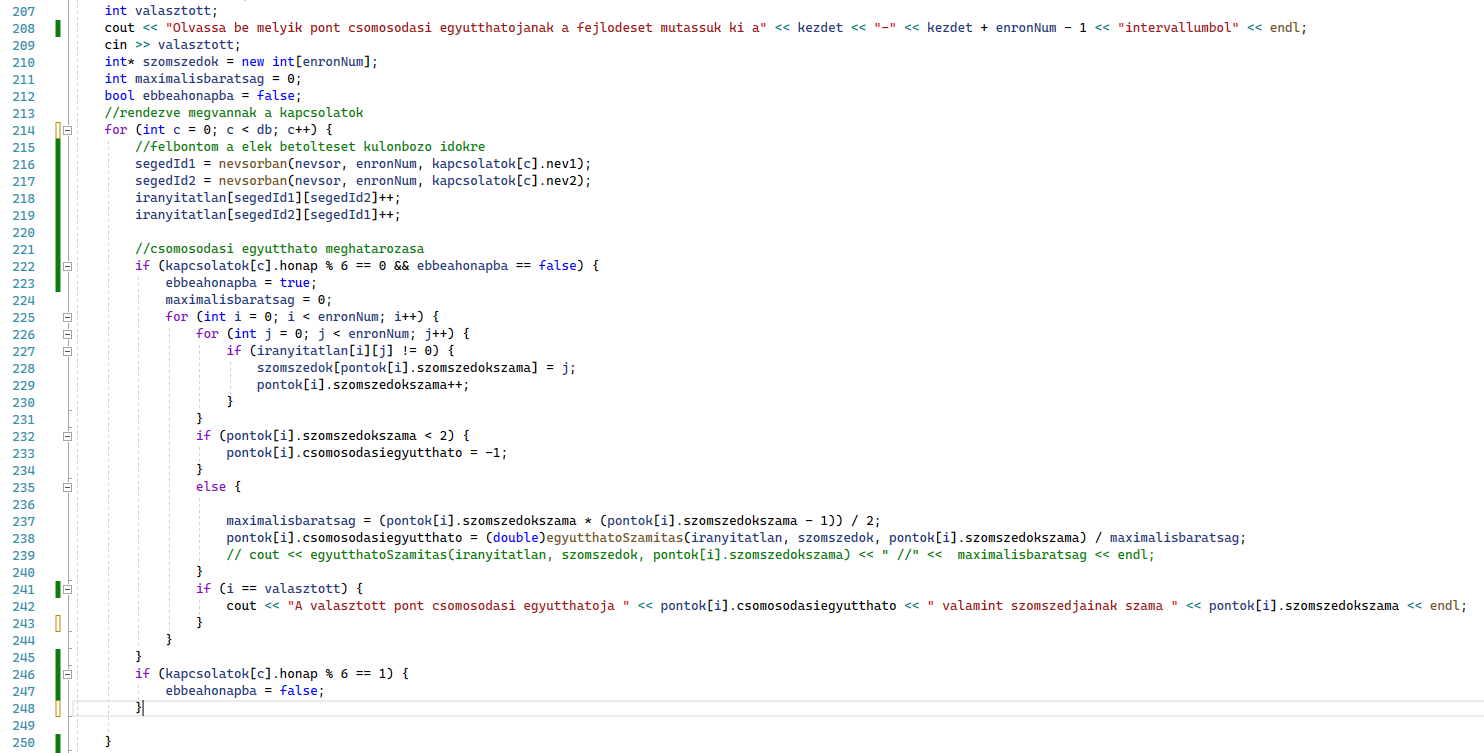
\includegraphics[scale=0.5 ]{images/egyutthato}
    \caption{Csomósodási együttható meghatározása időközönként}
    \label{fig:enter-label}
    \end{figure}

    A fenti kódrészletben a szűrésen és rendezésen áteső kapcsolatokat bejárva feltöltődik az irányítatlan gráf. Ez a feltöltés megszakad minden 6 hónapban, amikor a csomósodási pontok kiszámításai történnek. Ahhoz, hogy egy hónapban csak egyszer mérjünk, bevezettem az 'ebbenahonapba' nevű bool típusú változót, amely akkor vált igazra, ha már történt mérés az adott hónapban. Minden első és hetedik hónapban visszaállítom a változót hamisra (false). Az újbóli bejutás a mérésbe csak a 6-tal osztható hónapokban lehetséges.

Hogyan zajlik egy mérés? Egy mérés során megvizsgálom, hogy minden pontnak hány szomszédja van, és ezt beállítom az adott pontnak. Ezután két lehetőséget zárok ki: ha egy pontnak 1 vagy 0 szomszédja van. Ha egy pontnak 1 szomszédja van, akkor annak nem lehet más kapcsolata, és ha 0 szomszédja van, akkor sem lehet kiszámolni a pont csomósodási együtthatóját. Ha a szomszédok száma meghaladja az 1-et, akkor már kiszámítható az együttható.

    Az együttható meghatározásának képlete :
    \[
		Együttható=\leg\frac{Szomszédok Közötti Kapcsolatok Száma}{SzomszédokSzáma*(SzomszédokSzáma-1)/2}.
    \]

    Ugyanakkor beszéljek néhány használt függvényről és változóról. A program kezdetén bekérek egy 1 és 50 közötti számot, amely meghatározza a gráf méretét. Ez a változó neve 'enronNum' (210. sor). A szomszédok dinamikus tömböt használok, amelyben tárolom a pontok jelenlegi szomszédjait a kapcsolatok meghatározásához. A maximális barátság változó a fenti képletben látható osztó értékét fogja tárolni az eredmény számításához. A 'segedId1' és 'segedId2' változók a nevsorban függvény visszatérési értékét tárolják, amely egy int típusú elem lesz, mert a függvény visszaadja a nevsorban szereplő email indexét. Majd a meghatározott indexekből létrehozott éleket bevezetem az irányítatlan gráfot tartalmazó mátrixba. Ezzel már bemutattam az összes változót, amely a képen látható. Emellett említeném még a Kapcsolat típusú változót, amelyből egy tömb van létrehozva a kapcsolatok tárolására. Ennek az elemnek van két karakterláncot tartalmazó név1 és név2 változója, valamint egy három számból álló értéke a dátum kezelhetősége miatt.
    \begin{figure}[h]
        \centering
        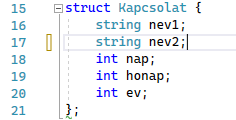
\includegraphics[scale=1]{images/kapcsolat}
        \caption{Kapcsolat struktúra}
        
    \end{figure}
    \item Utolsó megjegyzésként szeretném megmutatni egy algoritmus eredményét, amely egy 50 elemű gráf esetén, 3923 éllel rendelkezve az 5 pont csomósodási együtthatóját jeleníti meg 6 hónapos lépésekkel. Emellett a program végén meghatározom, melyik csúcs, vagyis személy rendelkezik a legnagyobb együtthatóval, feltéve, hogy a pontok számának legalább az ötödével van kapcsolatban. Végül, az utolsó eredményként meghatározom a legtöbb szomszéddal rendelkező személyt a gráfból.
    \begin{figure}[h]
        \centering
        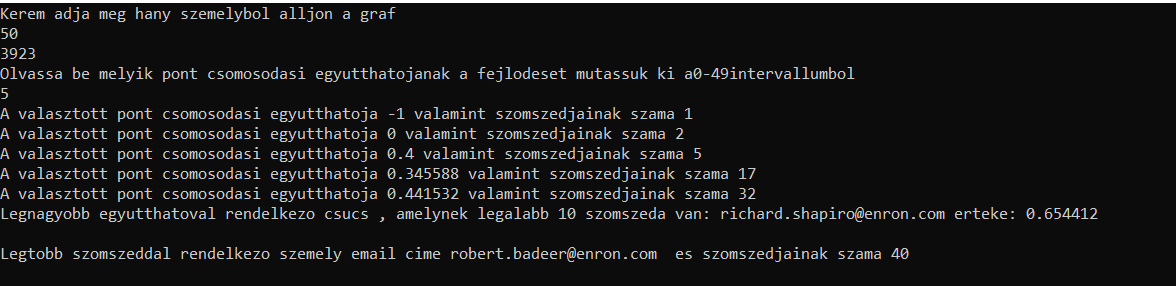
\includegraphics[scale=0.6]{images/eredmeny2}
        \caption{Változás az együtthatókban}
        
    \end{figure}
\end{itemize}

\section{Az hálózat kapcsolatainak vizsgálata}

Ebben a részben a kapcsolatok fontosságával foglalkoztam, és azt vizsgáltam, hogy egy kapcsolat, üzenetváltás mennyire fontos a hálózatban. Azért fontos egy ilyen nagy hálózatban, mert akár egyetlen egy kapcsolat, kötődés két egyén között is jelentős hatással lehet a hálózatra. Ha töröljük vagy megszüntetjük az adott kapcsolatot, az egész hálózat több részre szakadhat. Ezt a szétesést a gráfoknál úgy érhetjük el, hogy töröljük az egyik élt, amely egy hídat alkotott két komponens között.
\newpage

Az alábbi gráfon is látható , hogy a 3-1 él hídat képez a 2 háromszöget kirajzoló ponthalmazok között.
\begin{figure}[h]
    \centering
    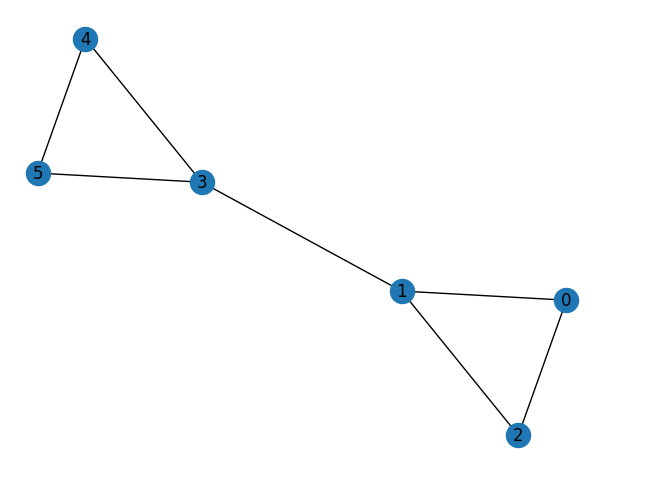
\includegraphics[scale=0.5]{images/hid}
    \caption{Gráf a híd magyarázatához}
    \label{fig:enter-label}
\end{figure}

A második ábrán megfigyelhető különbség segít megérteni a lokális híd kialakulásának könnyed magyarázatát. Amikor a 1-3 él törlésre kerül, még mindig képesek kommunikálni egymással az üzenetek, de a bejárás során megfigyeljük, hogy a két pont közötti távolság megnövekszik. Ha ez a növekedés meghaladja a 2 egységet, akkor a törölt élet lokális hídnak nevezzük.


\begin{figure}[h]
    \centering
    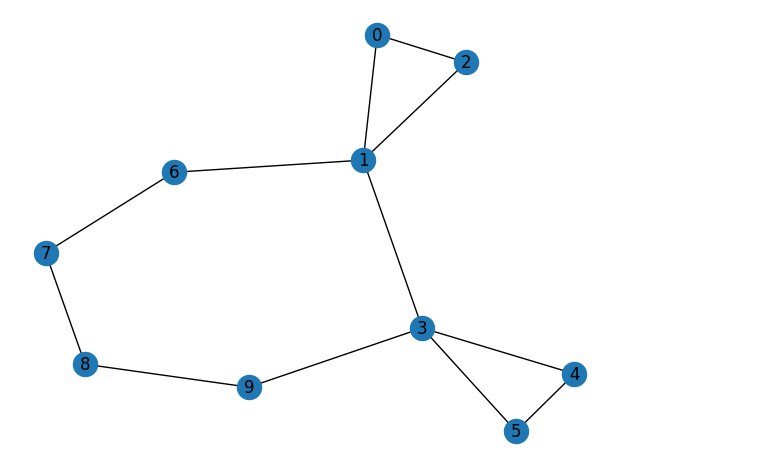
\includegraphics[scale=0.5]{images/lokalishid}
    \caption{Gráf a lokálishíd magyarázatához}
    \label{fig:enter-label}
\end{figure}
 
És mire is jó, ha tudjuk, hogy egy él híd vagy sem? A hídek lehetővé teszik két vagy több komponens összekapcsolását, így összefüggő gráfokkal tudunk dolgozni. Ugyanakkor a hídek nélkül is lehet az hálózat összefüggő, de ekkor lehetnek benne lokális hídek. Ha egy összefüggő gráfban nincs híd, és nincsenek lokális hídek sem, akkor nagy valószínűséggel teljes gráfról beszélünk.

Ezeket a jelenségeket vizsgáltam az általam használt adatokon, és a következő kis kódrészletekben bemutatom a kutatás lépéseit.

Az algoritmus legfontosabb eleme egy mélységi bejárás, amelyet a legrövidebb út meghatározásához is használtam a dolgozathoz szükséges szoftverek megírásában. A bejárás segítségével el tudom dönteni, hogy két pont között, ha törlöm az élt, akkor marad-e út a két csúcs között. Ennek egyik alapvető része az, hogy az irányított gráfot átalakítottam irányítatlan gráffá, mivel egy irányított gráfban nagyon nehéz két pont között több utat keresni, mivel kevesen válaszolnak az üzenetekre. Ezért szemléletesebbnek találtam, ha irányítatlan gráfon tesztelem a csúcsokat.

\begin{figure}[h]
    \centering
    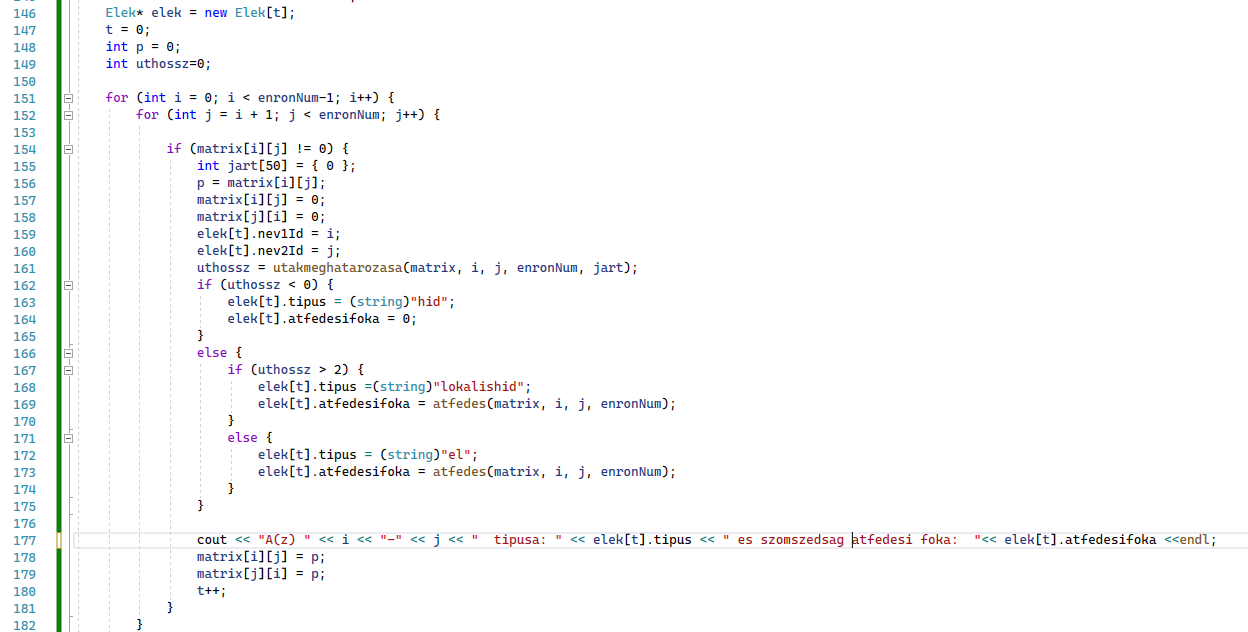
\includegraphics[scale=0.5]{images/hidprogram}
    \caption{Híd meghatározása}
    \label{fig:enter-label}
\end{figure}
 A fenti program részben megfigyelhető egy egymásba ágyazott 'for' ciklus, amely az éleket keresi meg és velük végzi el a műveleteket. Először megvizsgálja, hogy egy adott él létezik-e két pont között. Ha igen, akkor átírja annak értékét egy változóba, majd törli az élt (az értékét 0-ra állítja). A törölt éllel rendelkező mátrixszal meghívja a két pont közötti útvonalat kereső függvényt, amely egy számot ad vissza. Ha a visszatérített érték kisebb mint 0, akkor nincs kapcsolat a két pont között, tehát a törölt él híd volt. Ha az útvonal hossza meghaladja a 2 egységet, akkor a törölt élnek lokális híd jellegzetességet adunk. Ha az előző két eset nem teljesül, akkor az él átlagosnak tekintett jellegű marad.

Az élek tulajdonságainak tárolására egy Élek struktúrát hoztam létre, amely tartalmazza a küldő és címzett információkat, a szomszédsági átfedést, az él jellegét tároló lehetőséget, valamint a később említett köztességi fokszámát.


\begin{figure}[h]
    \centering
    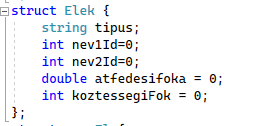
\includegraphics[scale=1.1]{images/elek}
    \caption{Él struktúra}
    \label{fig:enter-label}
\end{figure}

Ahogy az előző gondolatban is említésre került a következő tulajdonság amely az élekhez tartozik  a szomszédsági átfedés.Ezen változó kiszámítása hasonlóan a pontok csomósodási együtthatójához, egy olyan arány határoz meg, amely az él két végpontjának a közös szomszédjait és az mindkét pont összes szomszédjának számát használja fel.A kódrészlet magyarázata előtt kis ábrával pontosítanám ezen átfedetségi változó értékének fogalmát, melyben a pontok színbeli eltérésével szemléletesebb a különség és könnyen észrevehető , hogy miből is áll ez az érték.
\newpage

\begin{figure}[h]
    \centering
    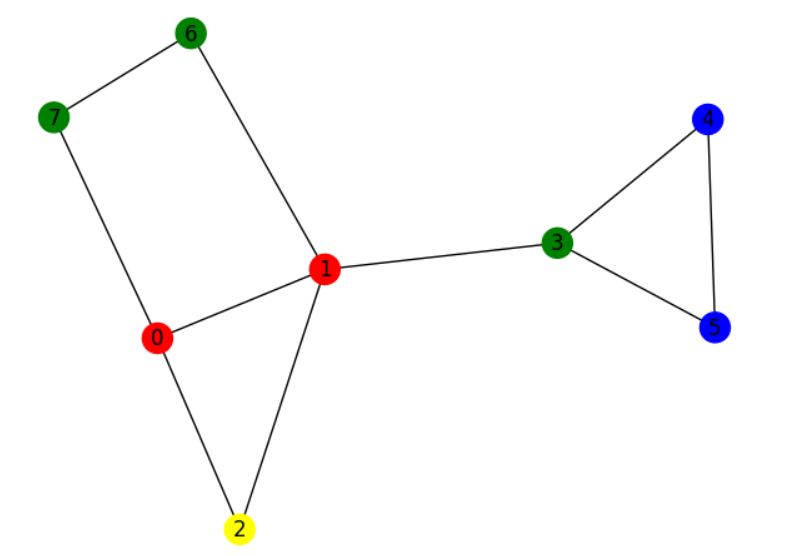
\includegraphics[scale=0.4]{images/atfedesi}
    \caption{Átfedéshez használt példa gráf}
    \label{fig:enter-label}
\end{figure}

Ahogy az előző részben is említésre került, az élekhez tartozik a szomszédsági átfedés tulajdonság. Ennek a változónak a kiszámítása hasonló módon történik, mint a pontok csomósodási együtthatójának meghatározása. Ez az arány meghatározza az él két végpontjának közös szomszédjainak számát és az összes szomszédjának számát mindkét pontnál. Az ábrával kísérve pontosítom ezen átfedési változó értékének fogalmát, ahol a pontok különböző színekkel vannak jelölve, hogy szemléletesebb legyen a különbség és könnyen észrevehető legyen, hogy ez az érték miből áll.

\begin{figure}[h]
    \centering
    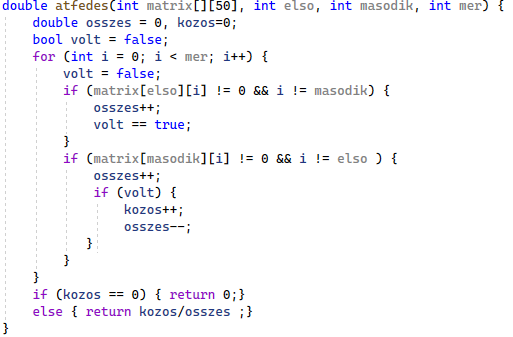
\includegraphics[scale=0.6]{images/atfedesikod}
    \caption{Átfedés számításához használt függvény}
    \label{fig:enter-label}
\end{figure}


A függvény paraméterlistája egy mátrixot tartalmaz, amelyben az élek vannak tárolva. A második paraméter az él indulási pontját határozza meg, és a függvény megvizsgálja ennek a pontnak a szomszédjait. Ezután a harmadik paraméterrel ismét ugyanezt a műveletet végzi el. Az utolsó paraméter meghatározza, hogy hány csúcsból áll a gráf. Ha ez a szám kevesebb, mint 50, akkor az "i" változónak nem kell 50-ig iterálnia a "for" ciklusban.

A közös szomszédok kiválasztása egy segéd "bool" típusú változóval van megoldva. Ez a változó csak akkor vesz fel igaz értéket, ha az "i"-dik csúcsnak van közös szomszédja az első elemmel. Ha a második elem is kapcsolatban van az "i"-dik elemmel, akkor azt közös szomszédnak számolom, és visszavonom az összes szomszéd számának növelését. A bejárás után, ha a közös változó értéke 0 maradt, akkor a függvény 0-t ad vissza, különben pedig egy 0 és 1 közötti értéket.

	%----------------------------------------------------------------------------
\chapter{Girvan-Newman módszer}
%----------------------------------------------------------------------------
\section{Általános tudnivaló a módszerről}

Az algoritmus elnevezése Michelle Girvan, egy amerikai fizikus, és Mark Newman, szintén egy amerikai fizikus nevéből származik. A két fizikus egy hierarchikus módszert fejlesztett ki a közösségek kimutatására komplex rendszerekben.

Az algoritmus a hálózat felépítését vizsgálja, és az élek közötti köztességi fokra épül. A köztességi fok egy érték, amely meghatározza, hogy az adott él hány legkisebb út megy át rajta. Ez az érték a forgalmat tükrözi, vagyis azt, hogy a legkisebb utak gyakori átjárhatósága mekkora. Az él közösségi fokának értéke az áthaladó összes legrövidebb út forgalmának az összege. Ez az érték segít több részre bontani a hálózatot a legforgalmasabb élek törlésével. Az így kapott részgráfok alkotják az első szintű gócokat. Ezután ezeket a részhalmazokat tovább lehet bontani, amíg minden élet törölünk.

Az általam megvalósított algoritmus három modulra épül. Az első modul az útmodul, amely a legrövidebb utak tárolásában használható, és képes az élek tárolására. A második modul az élekről tárol információkat, mint az él típusa, kezdő- és végpontja, köztességi foka és átfedési foka. Az utolsó modul azért jött létre, hogy egyik függvény visszatérési értékét tovább tudjuk adni, és ezen keresztül az éleket kezelni tudjuk.

\begin{figure}[h]
    \centering
    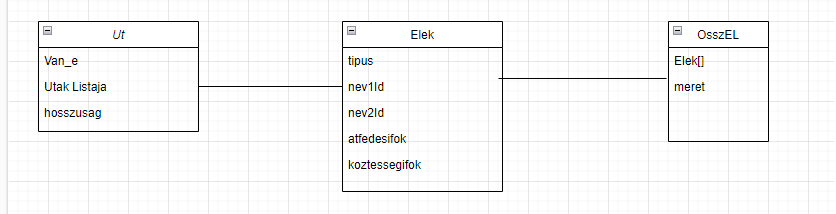
\includegraphics[scale=0.9]{images/modulok}
    \caption{Modulok}
    \label{fig:enter-label}
\end{figure}
\newpage
Modulok bemutatása után következzen a legkisebb út meghatározása :

\begin{figure}[h]
    \centering
    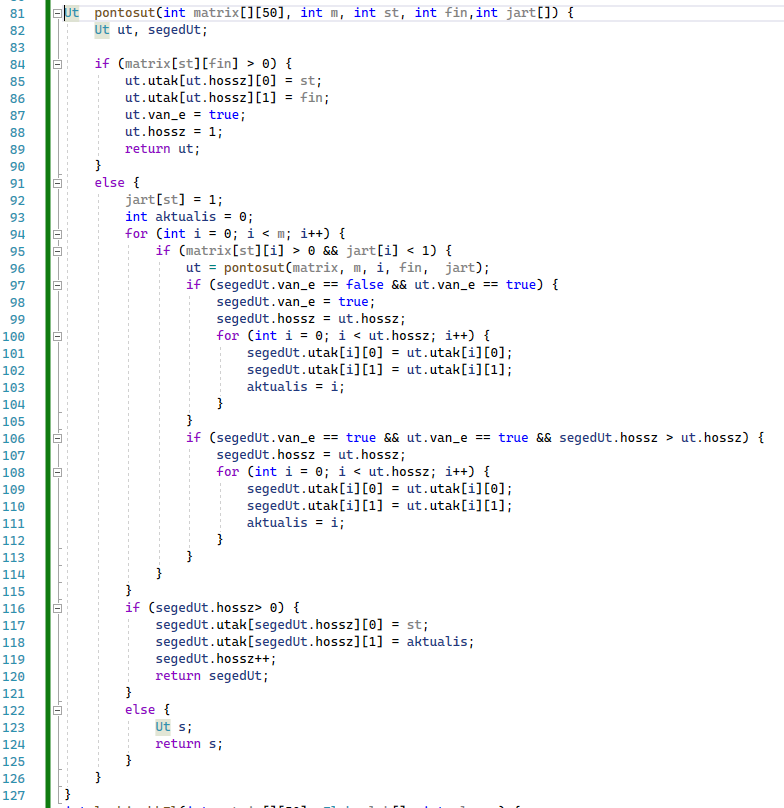
\includegraphics[scale=0.8]{images/pontosUt}
    \caption{Út meghatározására használt függvény}
    \label{fig:enter-label}
\end{figure}

Az algoritmusodban a legrövidebb utak meghatározásához szükséges az optimális útvonalak ismerete. Az élek közötti köztességi fok növelésével könnyen megtudhatod a keresett eredményt, ha pontosan ismered az irányt.

A fenti függvény meghatározza az adott út pontos éleit, és ehhez öt paramétert használ. Az első paraméter a gráf éleit tartalmazó mátrix, majd három 'int' típusú változó következik (a csúcsok száma, az indulási pont és a cél), végül pedig egy tömb, amelyben nyomon követed, hogy mely csúcsokon jártál már. A függvény első sorában létrehozol két 'Ut' típusú változót, amelyek a legjobb utat és a kapott értékeket tárolják a rekurzió során.

A függvény első ellenőrzése azt vizsgálja, hogy van-e kapcsolat az indulási pont és a cél között. Ha van kapcsolat, akkor hozzáadod az élek listáját a tárolt tömbhöz, beállítod a tömb méretét 1-re, és az "van-e ut" logikai változót igazra állítod. Ez az eset jelenti azt, amikor nem kell a függvényt újra meghívni, tehát itt véget ér a rekurzió, ha előzőleg elindult a folyamat.

A teljes függvény a rekurzióra épül, amely akkor hívja meg önmagát, ha nem kap rögtön választ, hanem tovább kell vizsgálnia. Ehhez megvizsgálod az indulási pont összes élét, hogy merre lehet továbbhaladni. Ezek az élek elvezetnek más pontokhoz, amelyekről szeretnéd megtudni, milyen messze vannak a céltól. Ez a folyamat addig ismétlődik, amíg egy vagy több megoldást találsz. Ha csak egy megoldás van, az lesz a legrövidebb út, de ha több van, akkor ki kell választanod a legjobbat. Ehhez szükséges a két változó, amelyeket az első sorban hoztál létre. Az élek listájának mérete kulcsfontosságú, mert ez döntő jelleggel befolyásolja a választ. Minél kisebb a legrövidebb út hossza, és ha valóban elértél a célhoz, annál jobb a megoldás. A ciklusban megkapod a legjobb utat, majd visszatérsz a függvényből egy kis bővítéssel. A bővítés azt jelenti, hogy hozzáadod az élt, amelyen keresztül eljutottál a legoptimálisabb szomszédhoz. Ebben az esetben növeled az élek listájának méretét, majd visszatérsz az így kapott úttal. Az így visszaadott értékek alapján beállítod az élek közötti köztességi fokot a következő függvényben.

\begin{figure}[h]
    \centering
    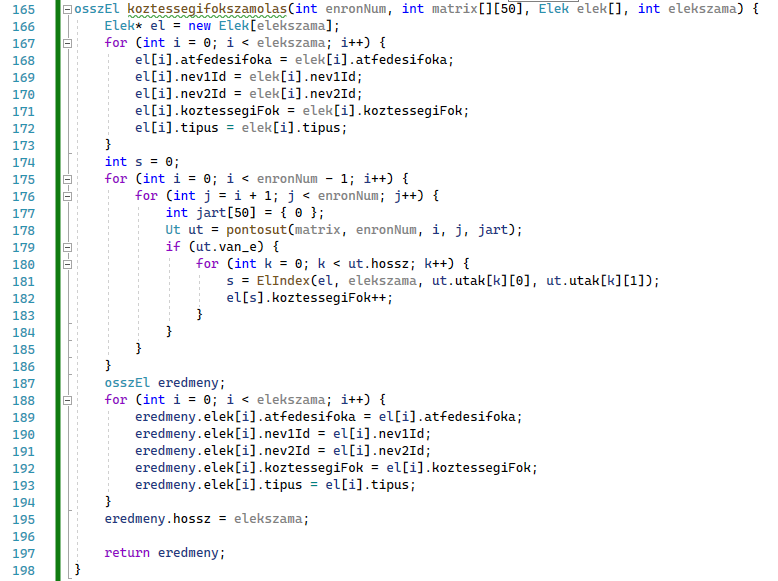
\includegraphics[scale=0.8]{images/koztessegifok}
    \caption{Köztességifok számítására alkalmazott függvény}
    \label{fig:enter-label}
\end{figure}

Ahogy látható, bejárom az összes lehetséges utat az egymásba ágyazott for ciklusok segítségével, és így meghatározom minden út pontos lépéseit. Ezeket az utakat aztán egy segédfüggvény (ElIndex) által feldolgozom, hogy növeljem az utakban előforduló élek köztessegi fokának számát. Ez a növelés akkor történik, ha az aktuális pontok között van út, mert a törlések és a komponensekre való szétesés megakadályozza, hogy minden pont között út létezzen. A köztessegi fok kiszámítása után az eredeti él listát visszatérítem, de a köztessegi fokokat átírom.

A következőkben bemutatom a Girvan-Newman módszer megvalósítását, amely segítségével meghatározom, hogy a legnagyobb azonos köztessegi fokkal rendelkező élek törlése során milyen gyorsan esik szét a gráf izolált pontokra.


\begin{figure}[h]
    \centering
    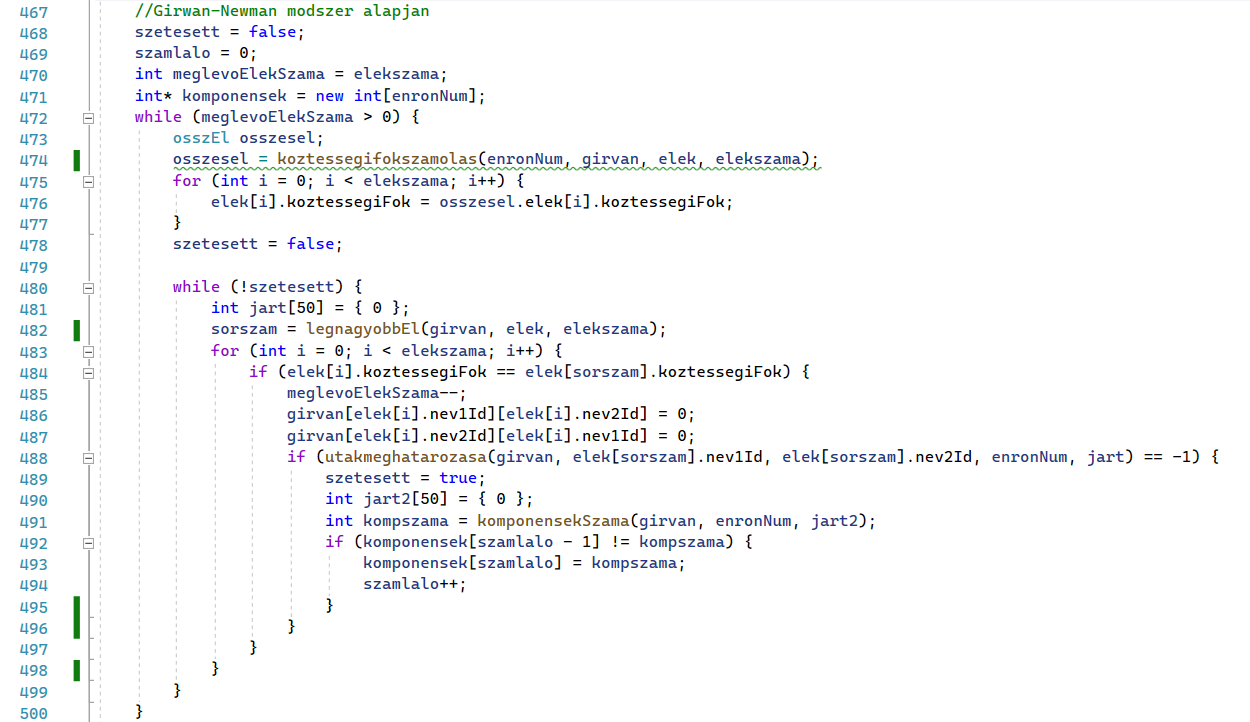
\includegraphics[scale=0.8]{images/girvan}
    \caption{Girvan-Newman módszer}
    \label{fig:enter-label}
\end{figure}

A fenti kódrészletben több egymásba ágyazott ciklus segítségével valósítom meg a műveleteket. Számolom a megmaradt éleket, amelyeket kitörlés esetén nullázok a girvan nevű mátrixon keresztül. A 488. sorban ellenőrzöm, hogy a törlés után van-e még út a törölt él két pontja között. Ha nincs, akkor biztosan változik a komponensek száma, amit később egy bejárás segítségével megszámolok és visszatérítek. Ha változik a komponensek száma, akkor visszalépek a kódrészlet elejére, újra számolom a köztessegi fokokat, majd ezt ismétlem addig, amíg elfogynak az élek.

Ezután felmerült bennem a kérdés, hogy vajon a súlyok szerinti élek törlése során nem szétesik-e hamarabb a gráf izolált csúcsokra. Ennek vizsgálatára elvégeztem a súlyok szerinti törlést csökkenő és növekvő sorrendben is. Minden művelet hasonlóan működött a Girvan-Newman algoritmushoz, hasonló ciklusokkal dolgoztam, és az eredmények is hasonlóak voltak, kis eltéréssel. A következő ábrákon látható eredmények rámutatnak arra, hogy a Girvan-Newman algoritmus a leggyorsabb módszer az összes él törlésére. Ugyanakkor, ha a súlyok kisebb szórásúak lennének, akkor véleményem szerint a gráf hamarabb szétesne a súly szerinti törlés esetén.

A következő lépésben a szoftver megjelenít egy kis adatvizualizációt, amely szemlélteti a hálózat kapcsolatainak törlés általi szétesését.
\begin{figure}[h]
    \centering
    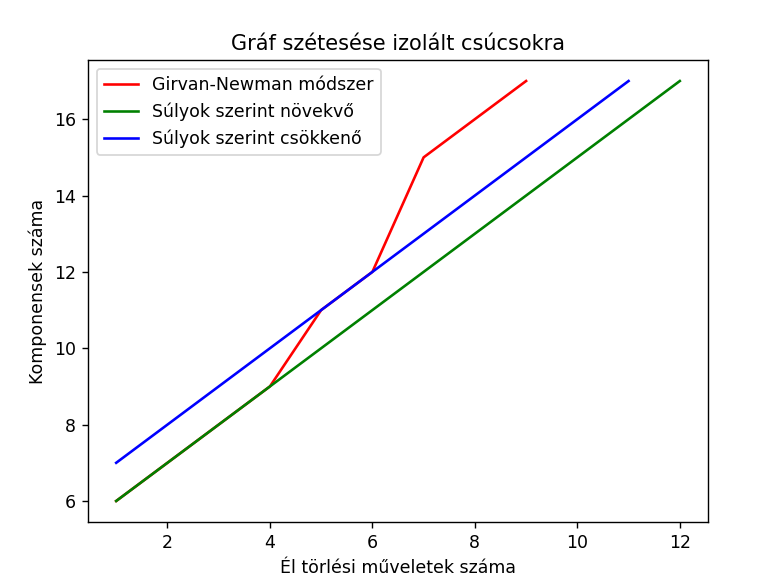
\includegraphics[scale=0.7]{images/hasonlitas}
    \caption{Összehasonlítás eredményének ábrázolása}
    \label{fig:enter-label}
\end{figure}


\begin{table}[h]
	\centering
	\begin{tabular}{ | l | c | c | c | c |}
		\hline 
		\textbf{Módszer} & \textbf{ciklusok száma} & \textbf{első éltörlés után}  \\
		\hline
		Girvan-Newman & $ 9 $ & $ 6 $  \\
		\hline
		Súlyokkal növekvő & $ 12 $ & $ 6 $ \\
		\hline
		Súlyokkal csökkenő & $ 11 $ & $ 7 $  \\
		\hline
		
	\end{tabular}
	\caption{Mérési eredmények  $ n = 17 $ csúccsal való tesztelésre.}
	\label{tablazat1}
\end{table}

A Girvan-Newman algoritmus a leggyorsabbnak bizonyult ebben az esetben, ahogy az összehasonlító ábrán is látható. Emellett bemutattam az egyes törlési események során készült állapotokat is.

A vizualizációs program lehetőséget nyújt arra, hogy válasszunk az 3 algoritmus által generált törlési események között, így kirajzolhatjuk a súlyok szerinti csökkenő vagy növekvő sorrendben bekövetkező változásokat.

Az alábbiakban megjelenítek egy állapotot, amelyet a súlyokkal való törlési művelet során generáltam:

\begin{itemize}
    \item  Az első három ábrán látható a Girvan-Newman módszer lépései által generált aktuális gráf. Ezek közül három ciklusos törlést mutatok be: az kezdeti állapotot, majd egy törlést és végül hét törlést követő állapotot. A fenti táblázatban is látható, hogy kilenc törlés után a gráf teljesen izolált csúcsokra bomlik. A két törlés azt jelzi, hogy a komponensek száma kettővel növekedett.
    \item  A második két ábrán a súlyok szerint növekvő sorrendben történik az élek kiválasztása és törlése.
    \item A táblázatban is látható, hogy a súly szerinti csökkenő és növekvő módszer nem dolgozik egyformán. Ha nem vesszük figyelembe a törlési módszer legfontosabb tulajdonságát, akkor azt gondolhatnánk, hogy a gráfban ugyanannyi különböző értékű él van, tehát mindegy, hogy lentről felfelé vagy fentről lefelé haladunk a súlyokkal, mindig ugyanannyi különböző súlyú él lesz. Úgy tűnhet, hogy nincs különbség a két módszer között. Azonban itt jön a fordulat, mert csak akkor lépünk tovább egy új lépésre, ha a törlések során a komponensek száma növekszik. Ezért a csökkenő és növekvő sorrendben történő módszer eredménye nem lesz azonos. Csak bizonyos speciális esetekben lesznek az eredmények azonosak, például ha az élek súlyai azonosak, vagy ha minden különböző súlyú él törlése több komponenst eredményez.      
\end{itemize}

\begin{figure}[h]
    \centering
    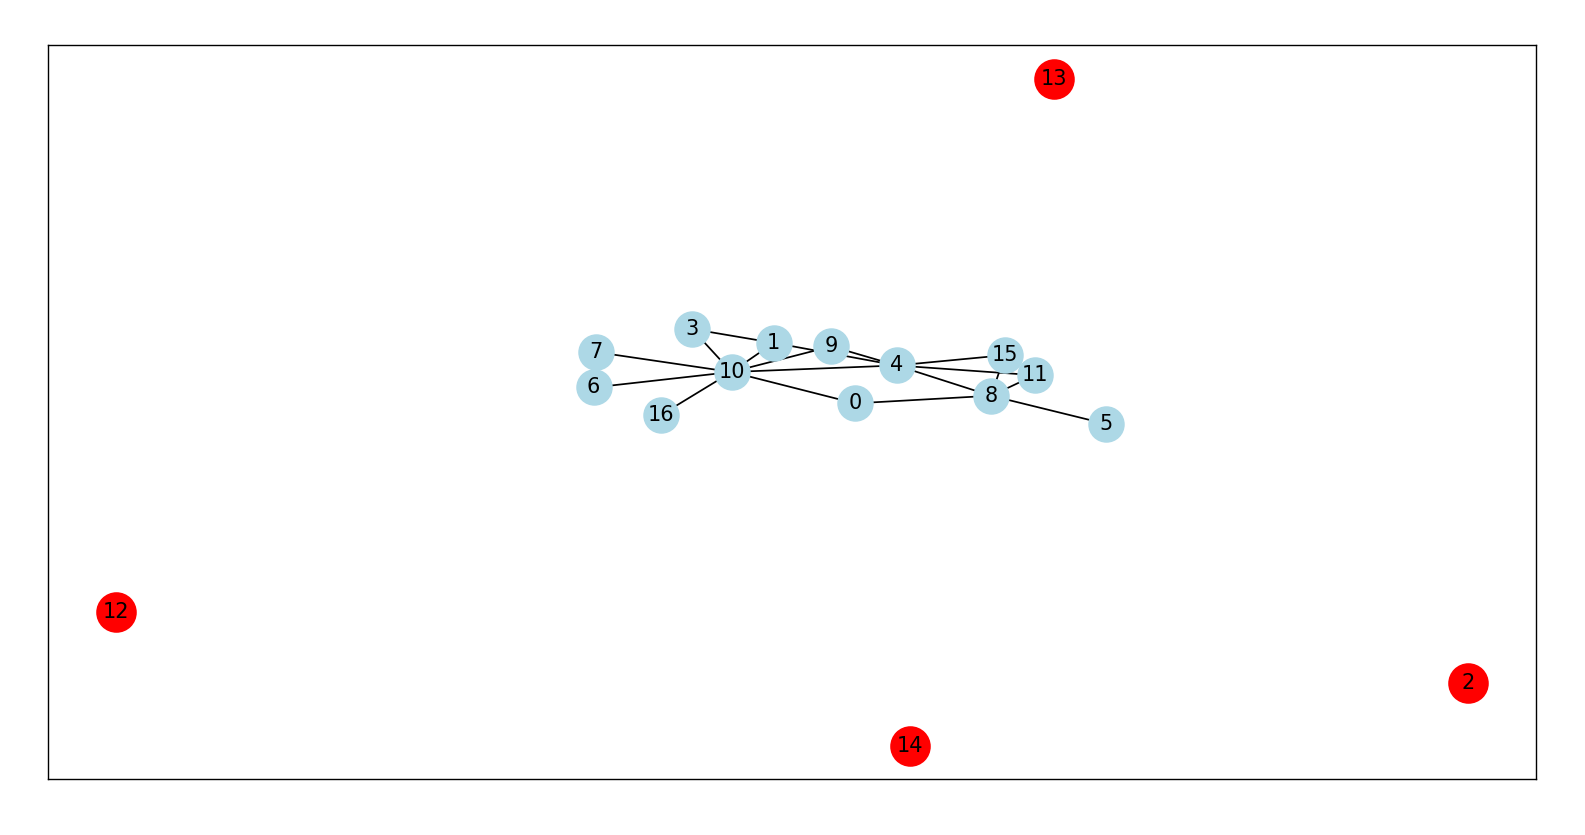
\includegraphics[scale=0.4]{images/girvan1lep}
    \caption{A gráf törlések előtt}
    \label{fig:enter-label}
\end{figure}


\begin{figure}[h]
    \centering
    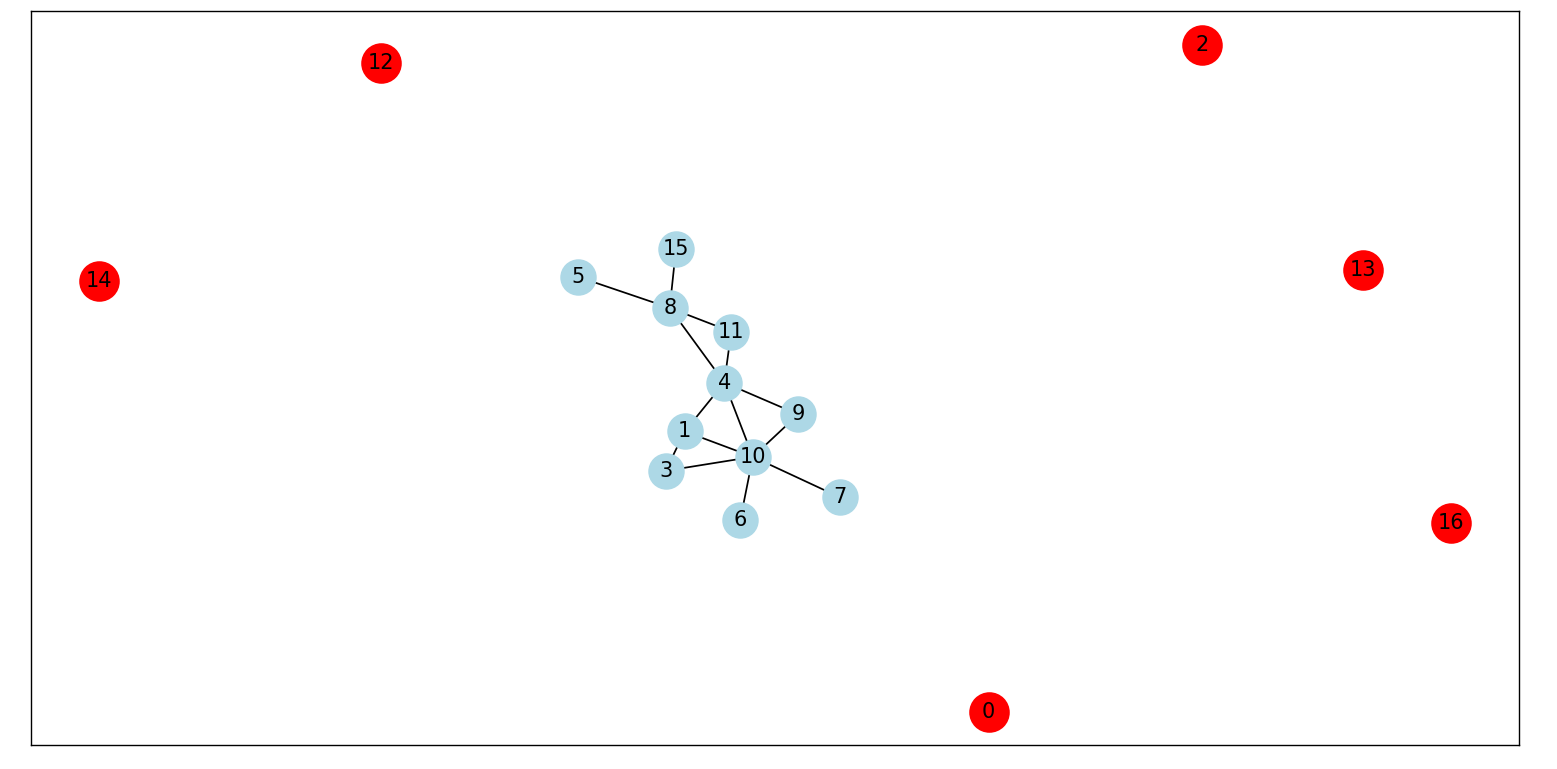
\includegraphics[scale=0.4]{images/girvan4lep}
    \caption{A gráf 2. Girvan-Newman módszerrel való törlés után }
    \label{fig:enter-label}
\end{figure}


\begin{figure}[h]
    \centering
    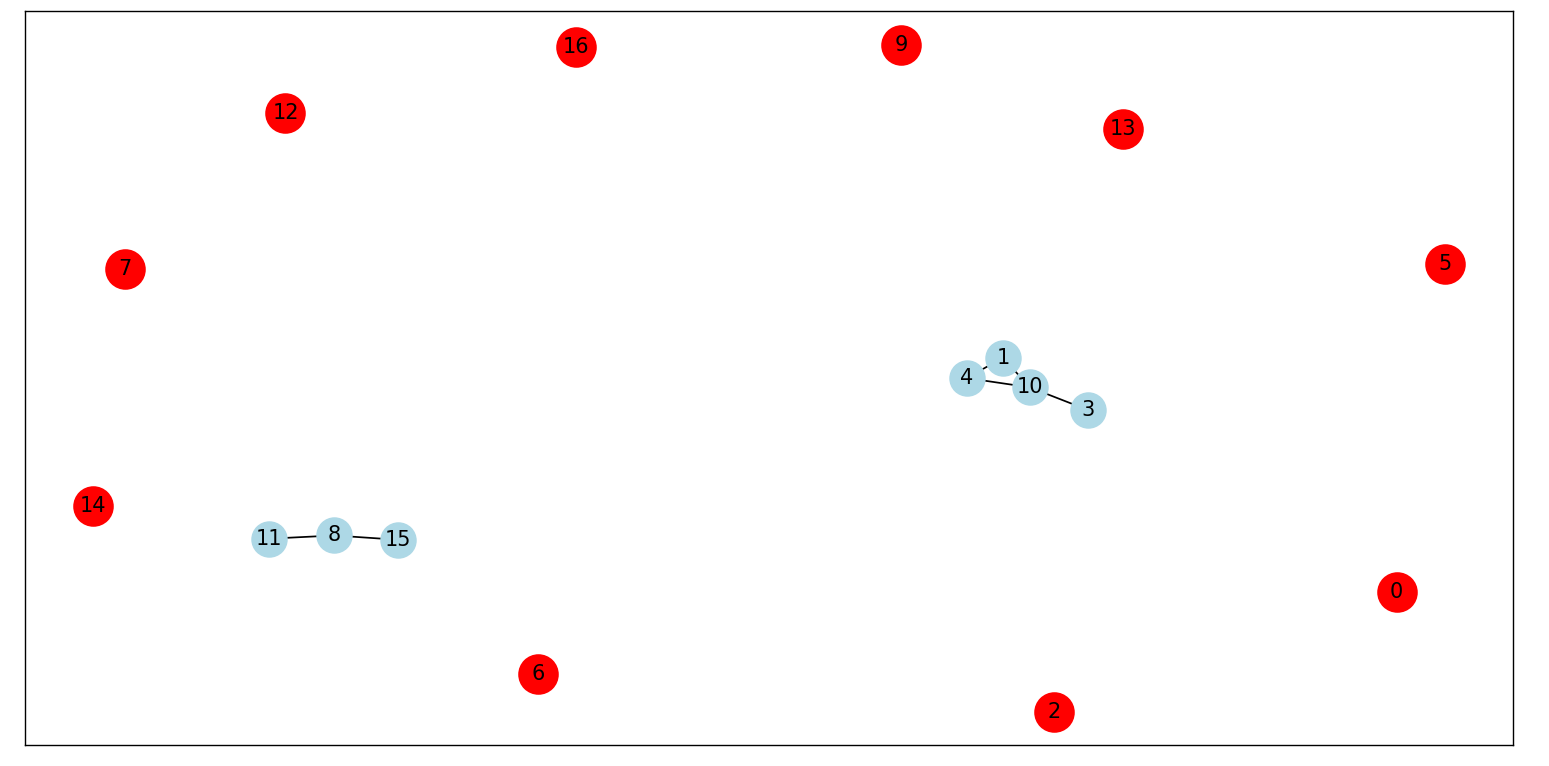
\includegraphics[scale=0.4]{images/girvan7lep}
    \caption{A gráf 7. Girvan-Newman módszerrel való törlés után}
    \label{fig:enter-label}
\end{figure}






\begin{figure}[h]
    \centering
    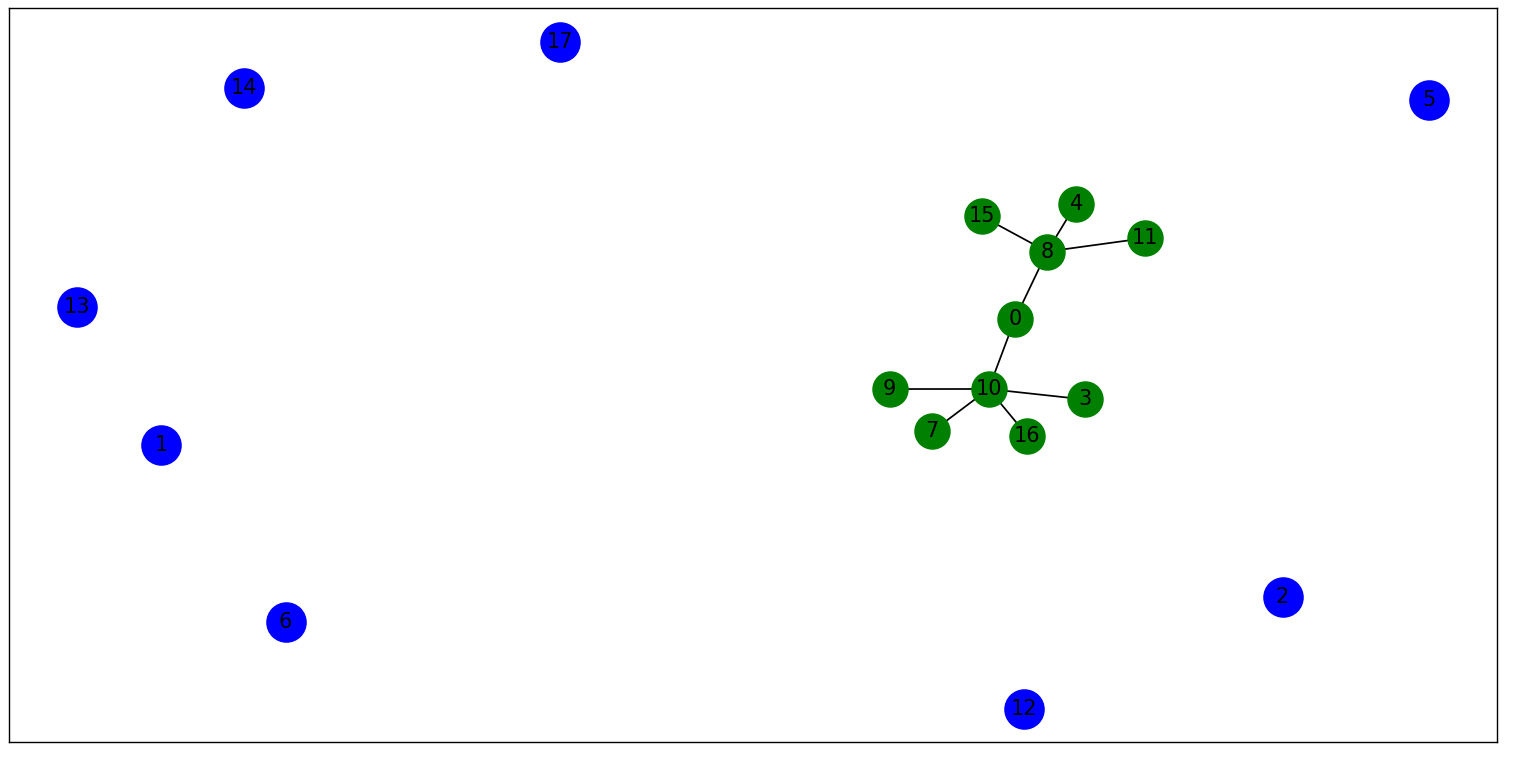
\includegraphics[scale=0.4]{images/suly5}
    \caption{A gráf 4 törlés után}
    \label{fig:enter-label}
\end{figure}


\begin{figure}[h]
    \centering
    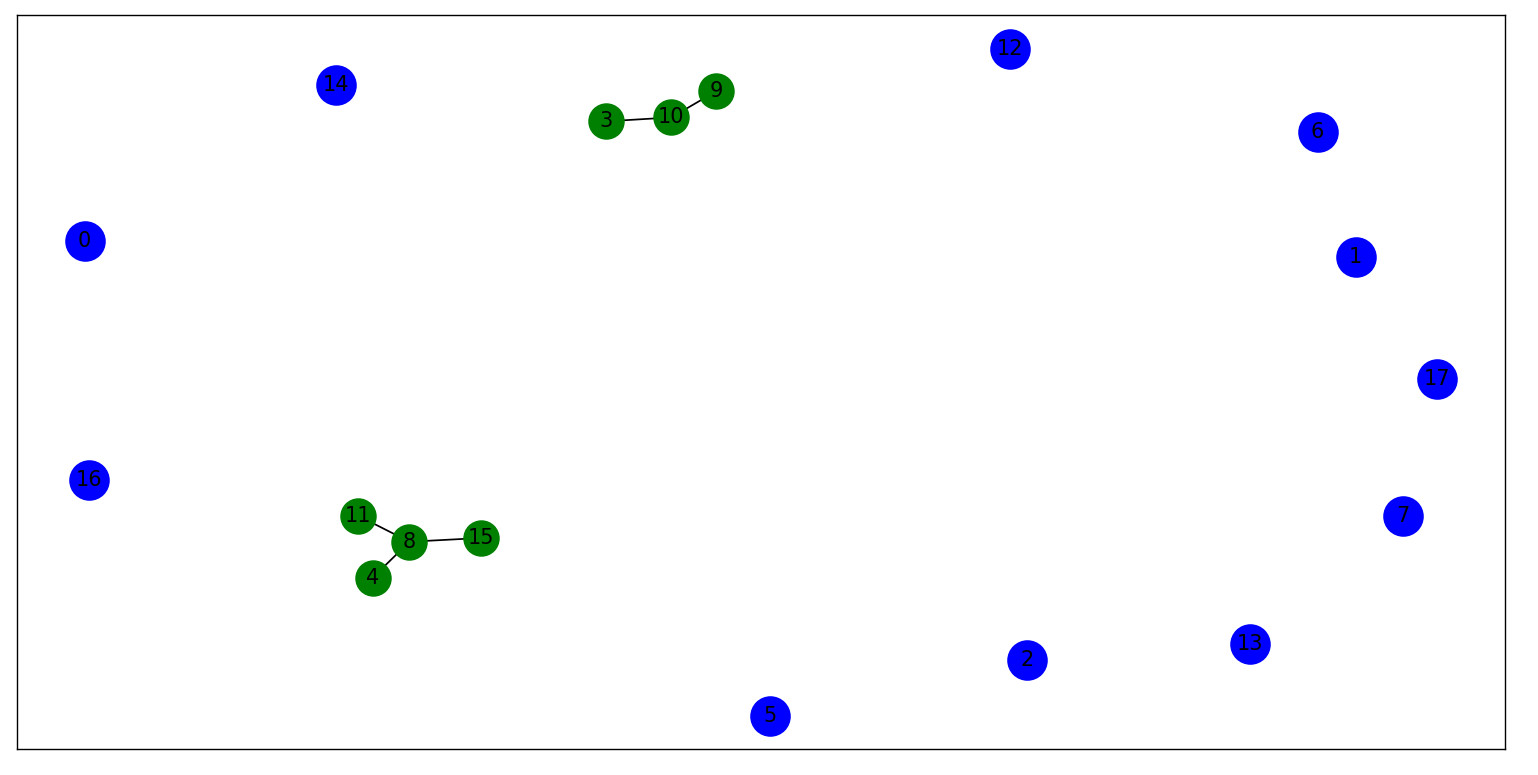
\includegraphics[scale=0.4]{images/suly9}
    \caption{A gráf 8 törlés után}
    \label{fig:enter-label}
\end{figure}




	%----------------------------------------------------------------------------
\chapter*{Összefoglaló}\addcontentsline{toc}{chapter}{Összefoglaló}
%----------------------------------------------------------------------------

Dolgozatomban több gráfelméleti algoritmust megírtam és teszteltem. Valós adatokkal feltöltött adatbázist használtam, amit kis adatbányászattal és adatszűréssel alakítottam könnyen használható formába. Az adatokat egy egyszerű szöveges állományban tároltam, ami segítségemre lesz a gráfelméleti algoritmusok gyakorlásában az egyetemi tananyag részére.

Az adatokat szűrtem és rendeztem, majd külön figyelmet fordítottam az adatvizualizációra is. Úgy gondolom, hogy ha látom a gráfokat, könnyebben tudom megérteni azokat, és könnyebb meghatározni egy adott algoritmus eredményét vagy a valós értékét. A Python programozási nyelvet használtam az adatbányászathoz, szűrésekhez és a vizualizációhoz. Fájlkezeléseket, néhány reguláris kifejezést és a matplotlib osztályt használtam az ábrák megjelenítéséhez.

Ezután áttértem egy másik programozási nyelvre, mert úgy gondolom, hogy ha a gráfelméletet C/C++ nyelven tanuljuk, könnyebben megérthetjük és átláthatjuk hasonló nyelven megírt kódokat, mint egy idegen nyelven írt algoritmust. C++ nyelven megvalósítottam az algoritmusaimat és szoftvereimet, amik a szociális jelenségekhez kapcsolódnak. Például, a pletyka terjedését vizsgáló algoritmust vagy a csomósodási együttható kiszámítását, amivel meghatározhatjuk, hogy mennyi esély van a barátok összekapcsolódására. Az irányított és irányítatlan gráfokat is figyelembe vettem, és bemutattam a változásokat az idő múlásával.

Az egyetemi órákon szereztem meg a gráfokkal kapcsolatos információkat és ismereteket.\cite{Katai}

Ezen kutatást, amelynek során vizsgálatokat végeztem, szeretném a jövőben továbbfejleszteni és magasabb szintre emelni. Az egyik célom ennek a fejlesztésnek a mesterséges intelligencia bevonása és az üzenetek hangulatának elemzése. Ezen túlmenően hosszabb távú terveim között szerepel a mesterséges intelligencia alkalmazása után az akkori üzenetek összehasonlítása a jelenlegi cégekben vagy akár kisebb szervezetekben elküldött e-mailekkel.

Github link: \url{https://github.com/tankotamas11/Allamvizsga2023}

% Koszonetnyilvanitas
%~~~~~~~~~~~~~~~~~~~~~~~~~~~~~~~~~~~~~~~~~~~~~~~~~~~~~~~~~~~~~~~~~~~~~~~~~~~~~~~~~~~~~~
	%----------------------------------------------------------------------------
\chapter*{\koszonetnyilvanitas}\addcontentsline{toc}{chapter}{\koszonetnyilvanitas}
%----------------------------------------------------------------------------

A szakdolgozatom elkészítéséhez nyújtott segítségért, a gráfelméleti gondolkodásom fejlesztéséhez nyújtott útbaigazitásokért valamint a dolgozat felépítéséhez átadott tanácsokért,ötletekért szeretnék köszönetet mondani a vezetőtanáraimnak, Dr. Kátai Zoltánnak és Oltean-Péter Borókának akik segítségével sok újat tanulhattam az elmúlt évben.Nagyon hálás vagyok tanáraimnak a téma ajánláshoz valamint a kezdeti adatbázis beszerzése is az ő érdemük ,mert ezáltal megteremtettek egy alapanyagot amin elvégezhettem számos műveletet , ennek köszönhetően fejleszthettem az algoritmikai tudásomat.


Utolsó gondolatként remélem sikeresen felhasználhatóak lesznek ezen algoritmusok és vizualizációk a jövő generációk tanításához , melynek ötletadója Dr. Kátai Zoltán tanárúr volt .Örömmel töltött el , hogy segíthetek a következő hallgatóknak a gráfelméleti tananyag vizualizációkkal való fejlesztésemmel ,hisz fontos célként tűzhettem ki magam előtt ezen gonolatot ami egy plusz motivációt adott a dolgozat elkészítéséhez.


% Tablazatok es abrak jegyzeke (EZ NEM KOTELEZO)
%~~~~~~~~~~~~~~~~~~~~~~~~~~~~~~~~~~~~~~~~~~~~~~~~~~~~~~~~~~~~~~~~~~~~~~~~~~~~~~~~~~~~~~
	\listoffigures\addcontentsline{toc}{chapter}{\abrakjegyzeke}
	\listoftables\addcontentsline{toc}{chapter}{\tablazatokjegyzeke}


% Bibliography
%~~~~~~~~~~~~~~~~~~~~~~~~~~~~~~~~~~~~~~~~~~~~~~~~~~~~~~~~~~~~~~~~~~~~~~~~~~~~~~~~~~~~~~
	\bibliography{mybib}
	\addcontentsline{toc}{chapter}{\irodalomjegyzek}
	\bibliographystyle{alpha}
	
% Appendix
%~~~~~~~~~~~~~~~~~~~~~~~~~~~~~~~~~~~~~~~~~~~~~~~~~~~~~~~~~~~~~~~~~~~~~~~~~~~~~~~~~~~~~~
	%\include{appendices}

\label{page:last}
\end{document}
